\documentclass[12pt]{article}
\usepackage[a4paper, total={15cm,25cm}]{geometry}
\usepackage{titlesec}
\usepackage{graphicx}
\usepackage{float}
\usepackage{hyperref}
%\usepackage{fancyhdr}
%\setlength{\headheight}{15pt}
%\pagestyle{empty}
%\fancyhead[L]{110-1 Bio-MEMS Fabrication Homework}
%\fancyhead[R]{鄭泊聲 b07611002}
\usepackage{amsmath}
\usepackage{latexsym}
\usepackage{multirow}
\graphicspath{ {./images/} }
\usepackage[backend=biber, citestyle=numeric, bibstyle=numeric, sorting=none]{biblatex}
\addbibresource{ref.bib}
\usepackage{mathspec}   %加這個就可以設定字體
\usepackage{xeCJK}       %讓中英文字體分開設置
\setCJKmainfont{Noto Serif CJK TC} %設定中文為系統上的字型
\newCJKfontfamily[chineseSans]\CJKsans{Noto Sans CJK TC}
\setmainfont{Sabon}
\setsansfont{IBM Plex Sans}
\setmonofont{Roboto Mono}
\XeTeXlinebreaklocale "zh"             %這兩行一定要加,中文才能自動換行
\XeTeXlinebreakskip = 0pt plus 1pt     %這兩行一定要加,中文才能自動換行
\renewcommand{\baselinestretch}{1.35}
\renewcommand{\figurename}{圖}
\renewcommand{\tablename}{表}
\renewcommand{\abstractname}{摘要}
\renewcommand{\contentsname}{目錄}
\renewcommand{\listtablename}{表格目錄}
%\renewcommand*{\bibfont}{\footnotesize}
\titleformat*{\section}{\Large \bfseries}
\titleformat*{\subsection}{\large \bfseries}
\titleformat*{\subsubsection}{\bfseries}
%\setcounter{tocdepth}{2}

\title{Development of HyperSpectral Imaging system}
\author{鄭泊聲\thanks{College Student Researcher, Center for Condensed Matter Science, National Taiwan University}
\and 指導教授:張玉明\thanks{Distinguished Research Fellow, Center for Condensed Matter Science, National Taiwan University}}

\date{\today}

\begin{document}
    \maketitle
    \tableofcontents
    \section{第一階段: 硬體}
    第一階段系統是為了在巨觀尺度下觀測實域影像而設計,在本計畫中也是作為概念驗證與軟體開發的雛型。
    在這個階段中,整個系統主要由以下幾個部建構成:
    \begin{enumerate}
        \item Specim V10E 線光譜儀
                \begin{itemize}
                    \item 搭配 Specim OLE 23(mm) 物鏡
                    \item 光譜範圍: 400-1000 $nm$
                    \item 入射狹縫寬: 30 $\mu m$
                    \item 成像尺寸: Image size: $6.15(spectral) \times 14.2 mm$
                \end{itemize}
        \item Andor iXon DU897 EMCCD
            \begin{itemize}
                \item 512 $\times$ 512 pixels
                \item 8.2 $\times$ 8.2 mm
                \item TE cooler
                \item Electron Multiplying gain
            \end{itemize}  
        \item Suruga Seiki 電動載台
                \begin{itemize}
                    \item 搭配 D120 控制器
                \end{itemize}
    \end{enumerate}
    由於V10E線光譜儀的成像尺寸與iXon的正方形CCD尺寸並不同,因此當兩部儀器接合使用後,有部分的像是我們無法觀測到的,如圖\ref{figure: image size}所示,
    我們將能在系統中能到看到V10E的整個光譜範圍,但觀測物的Y軸方向,卻因為iXon CCD的高度較小,因此無法完整觀測。

    \begin{figure}[t]
        \centering
        \includegraphics[width=0.5\linewidth]{imagesize.jpg}
        \caption{Image size when combined}
        \label{figure: image size}
    \end{figure}

    \begin{figure}[t]
        \centering
        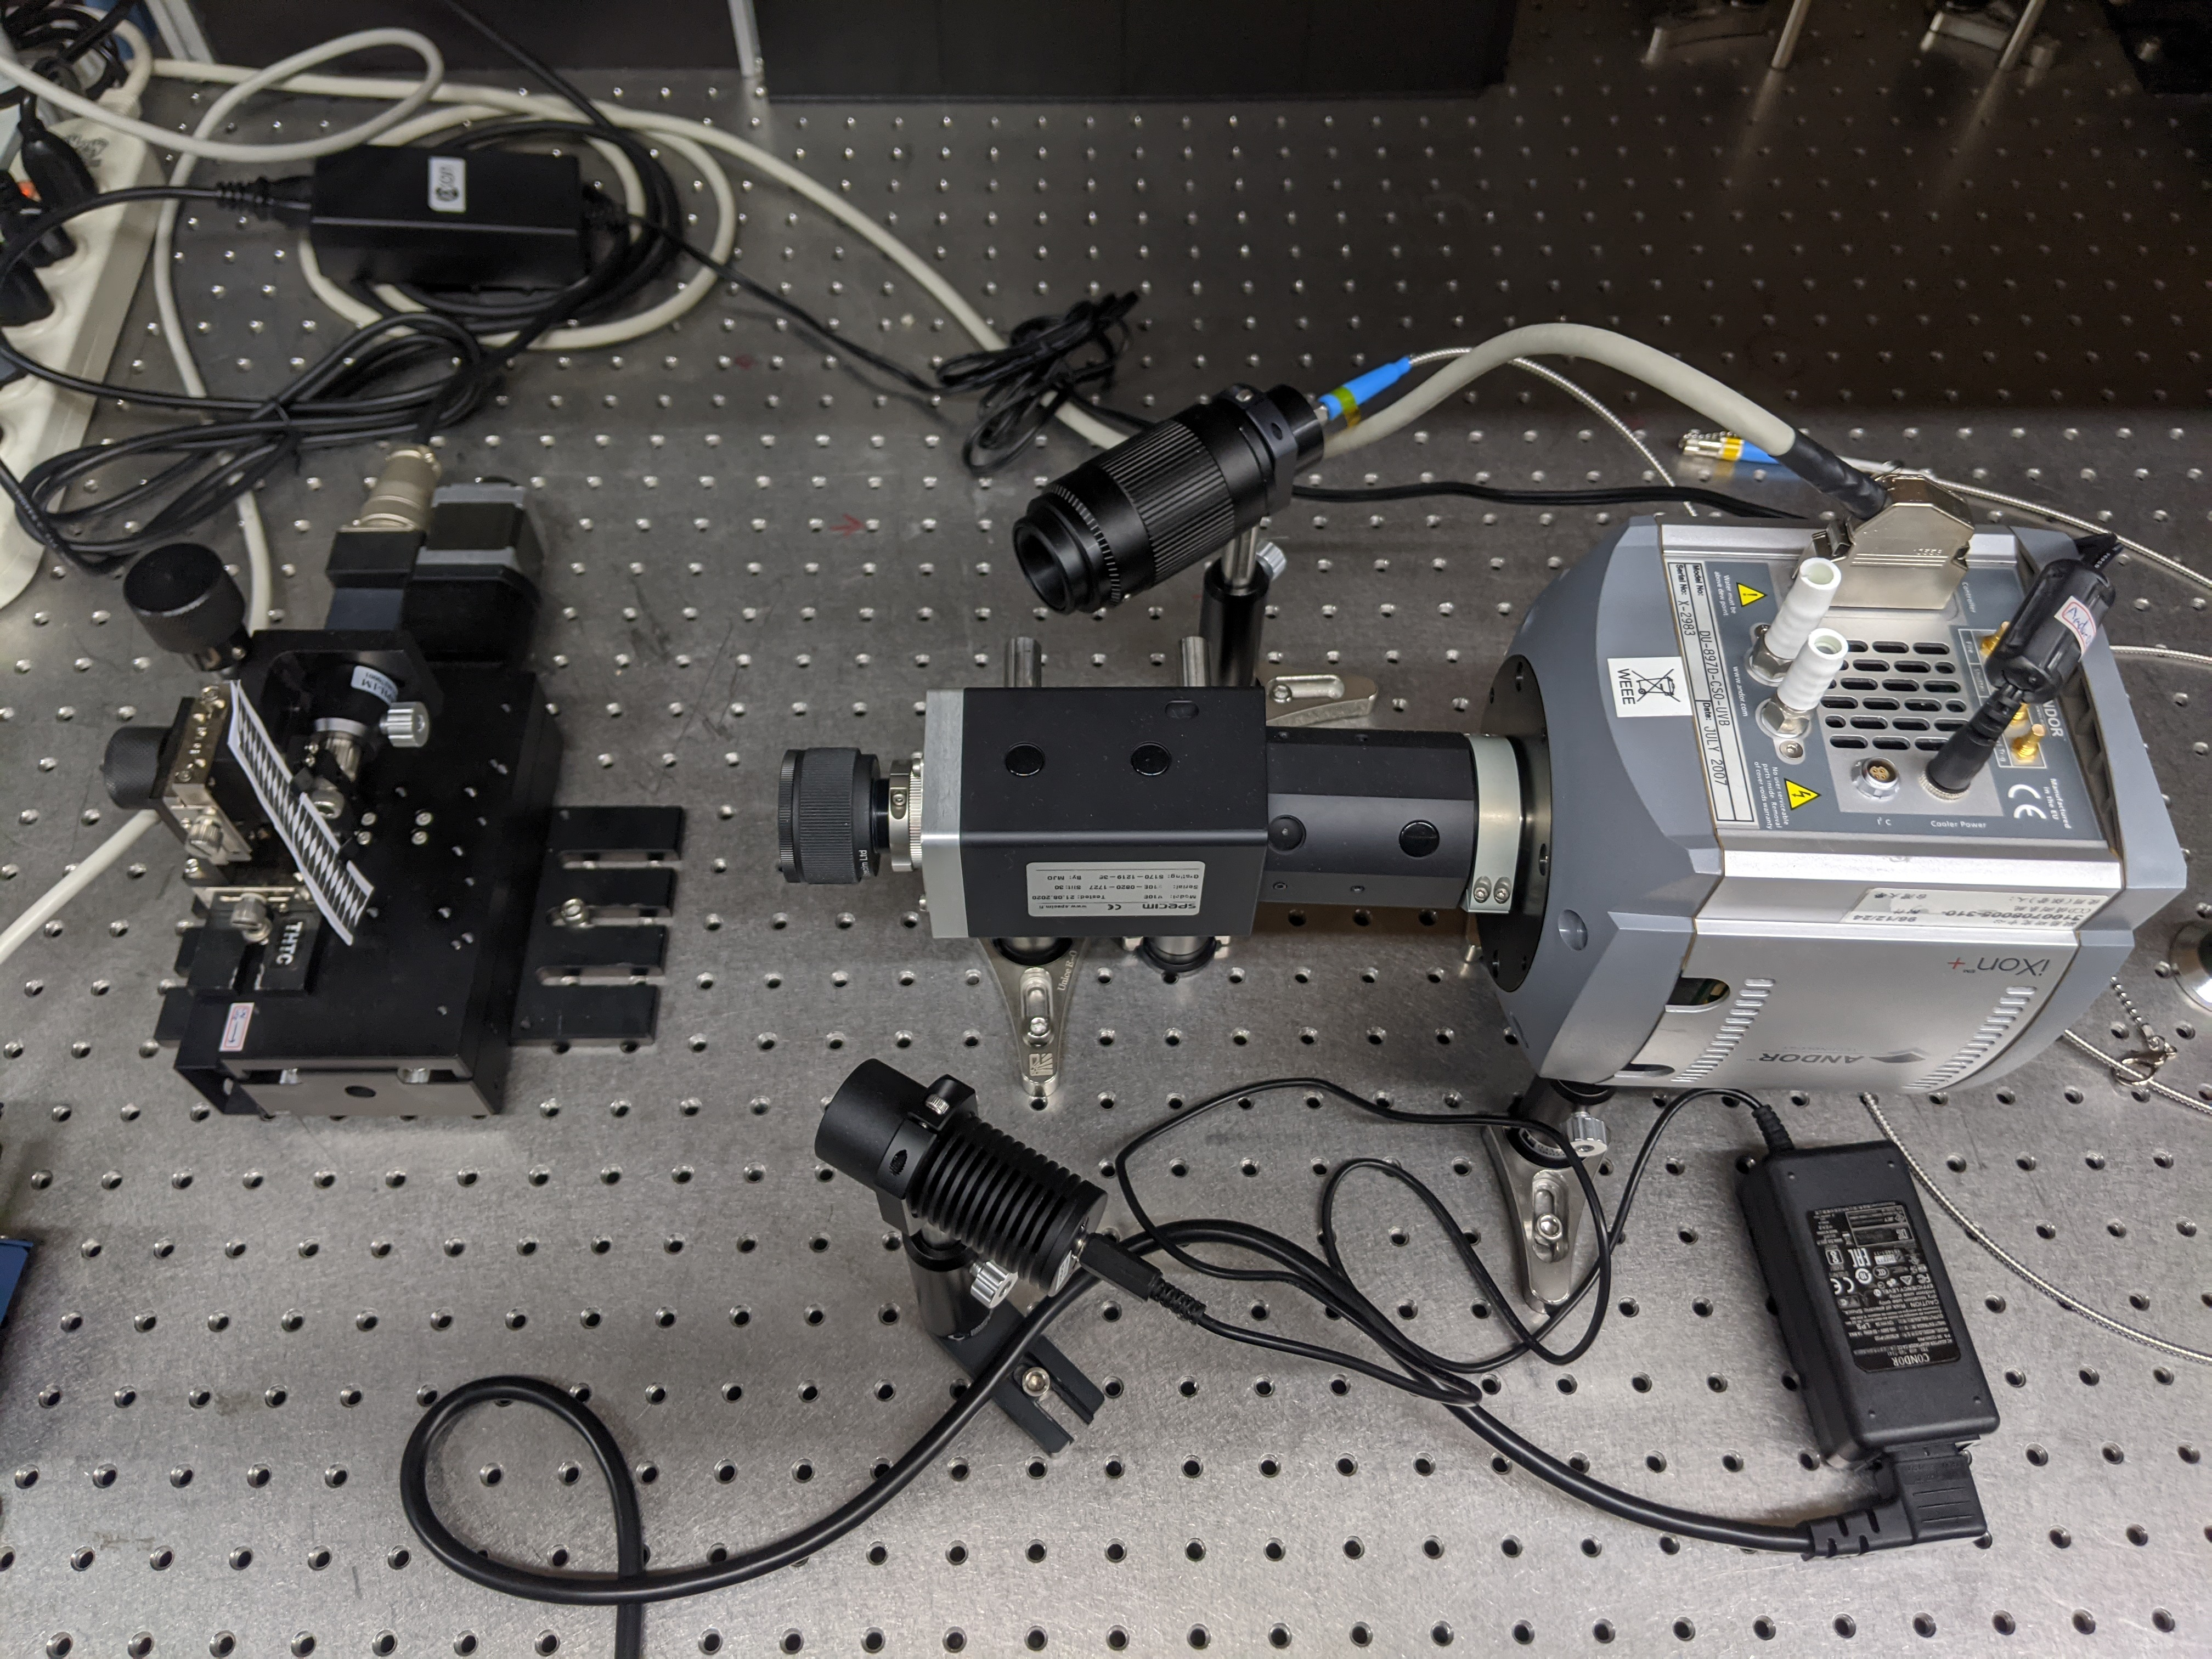
\includegraphics[width=0.65\linewidth]{PXL_20210723_094307842.jpg}
        \caption{Stage, spectrograph, ccd}
        \label{figure: 1 stage setup}
    \end{figure}
    
    圖\ref{figure: 1 stage setup}呈現出第一階段系統的樣貌,在照片中另外可以看到LED光源,從外部的黑色手電筒照射觀測物。

    \subsection{組裝對正與對焦}
    將iXon相機與V10E線光譜儀組裝接合時,有兩件事情必須確認,才能確保所擷取到的影像是正向且準焦的。
    首先,必須確認V10E的像正好在iXon的CCD上匯聚成像。調整方法是,在兩部儀器接合和後,未裝上物鏡的情形下,從線光譜儀的入射狹縫
    ,以一個標準光源打入光線(如我使用Ocean optics Cal-2000 Mercury-Argon 校正用光源),並在電腦上觀測iXon的即時影像。此時由於線光譜儀的入射狹縫完全被標準光源所照亮,
    在影像的畫面上應該看見一條條的直線,每個直線就是光源的一個光譜線。此時即可前後調整V10E後端的鏡組位置(圖\ref{figure: specim bfp lens}),
    直到畫面上的光譜線變得最細、最銳利之時,就代表已經將線光譜儀的像準確成在CCD上了。

    接著,要確保兩部儀器之間的對正,使像跟CCD的方向對齊。只要看畫面上的直線是否完全垂直,就能知道像的方向是否對齊,若直線有傾斜,就要調整V10E與iXon之間的接合角度。以上兩項接合對正都完成後,畫面上的影像應該如圖\ref{figure: align v10e and ixon}所示。

    \begin{figure}[t]
        \centering
        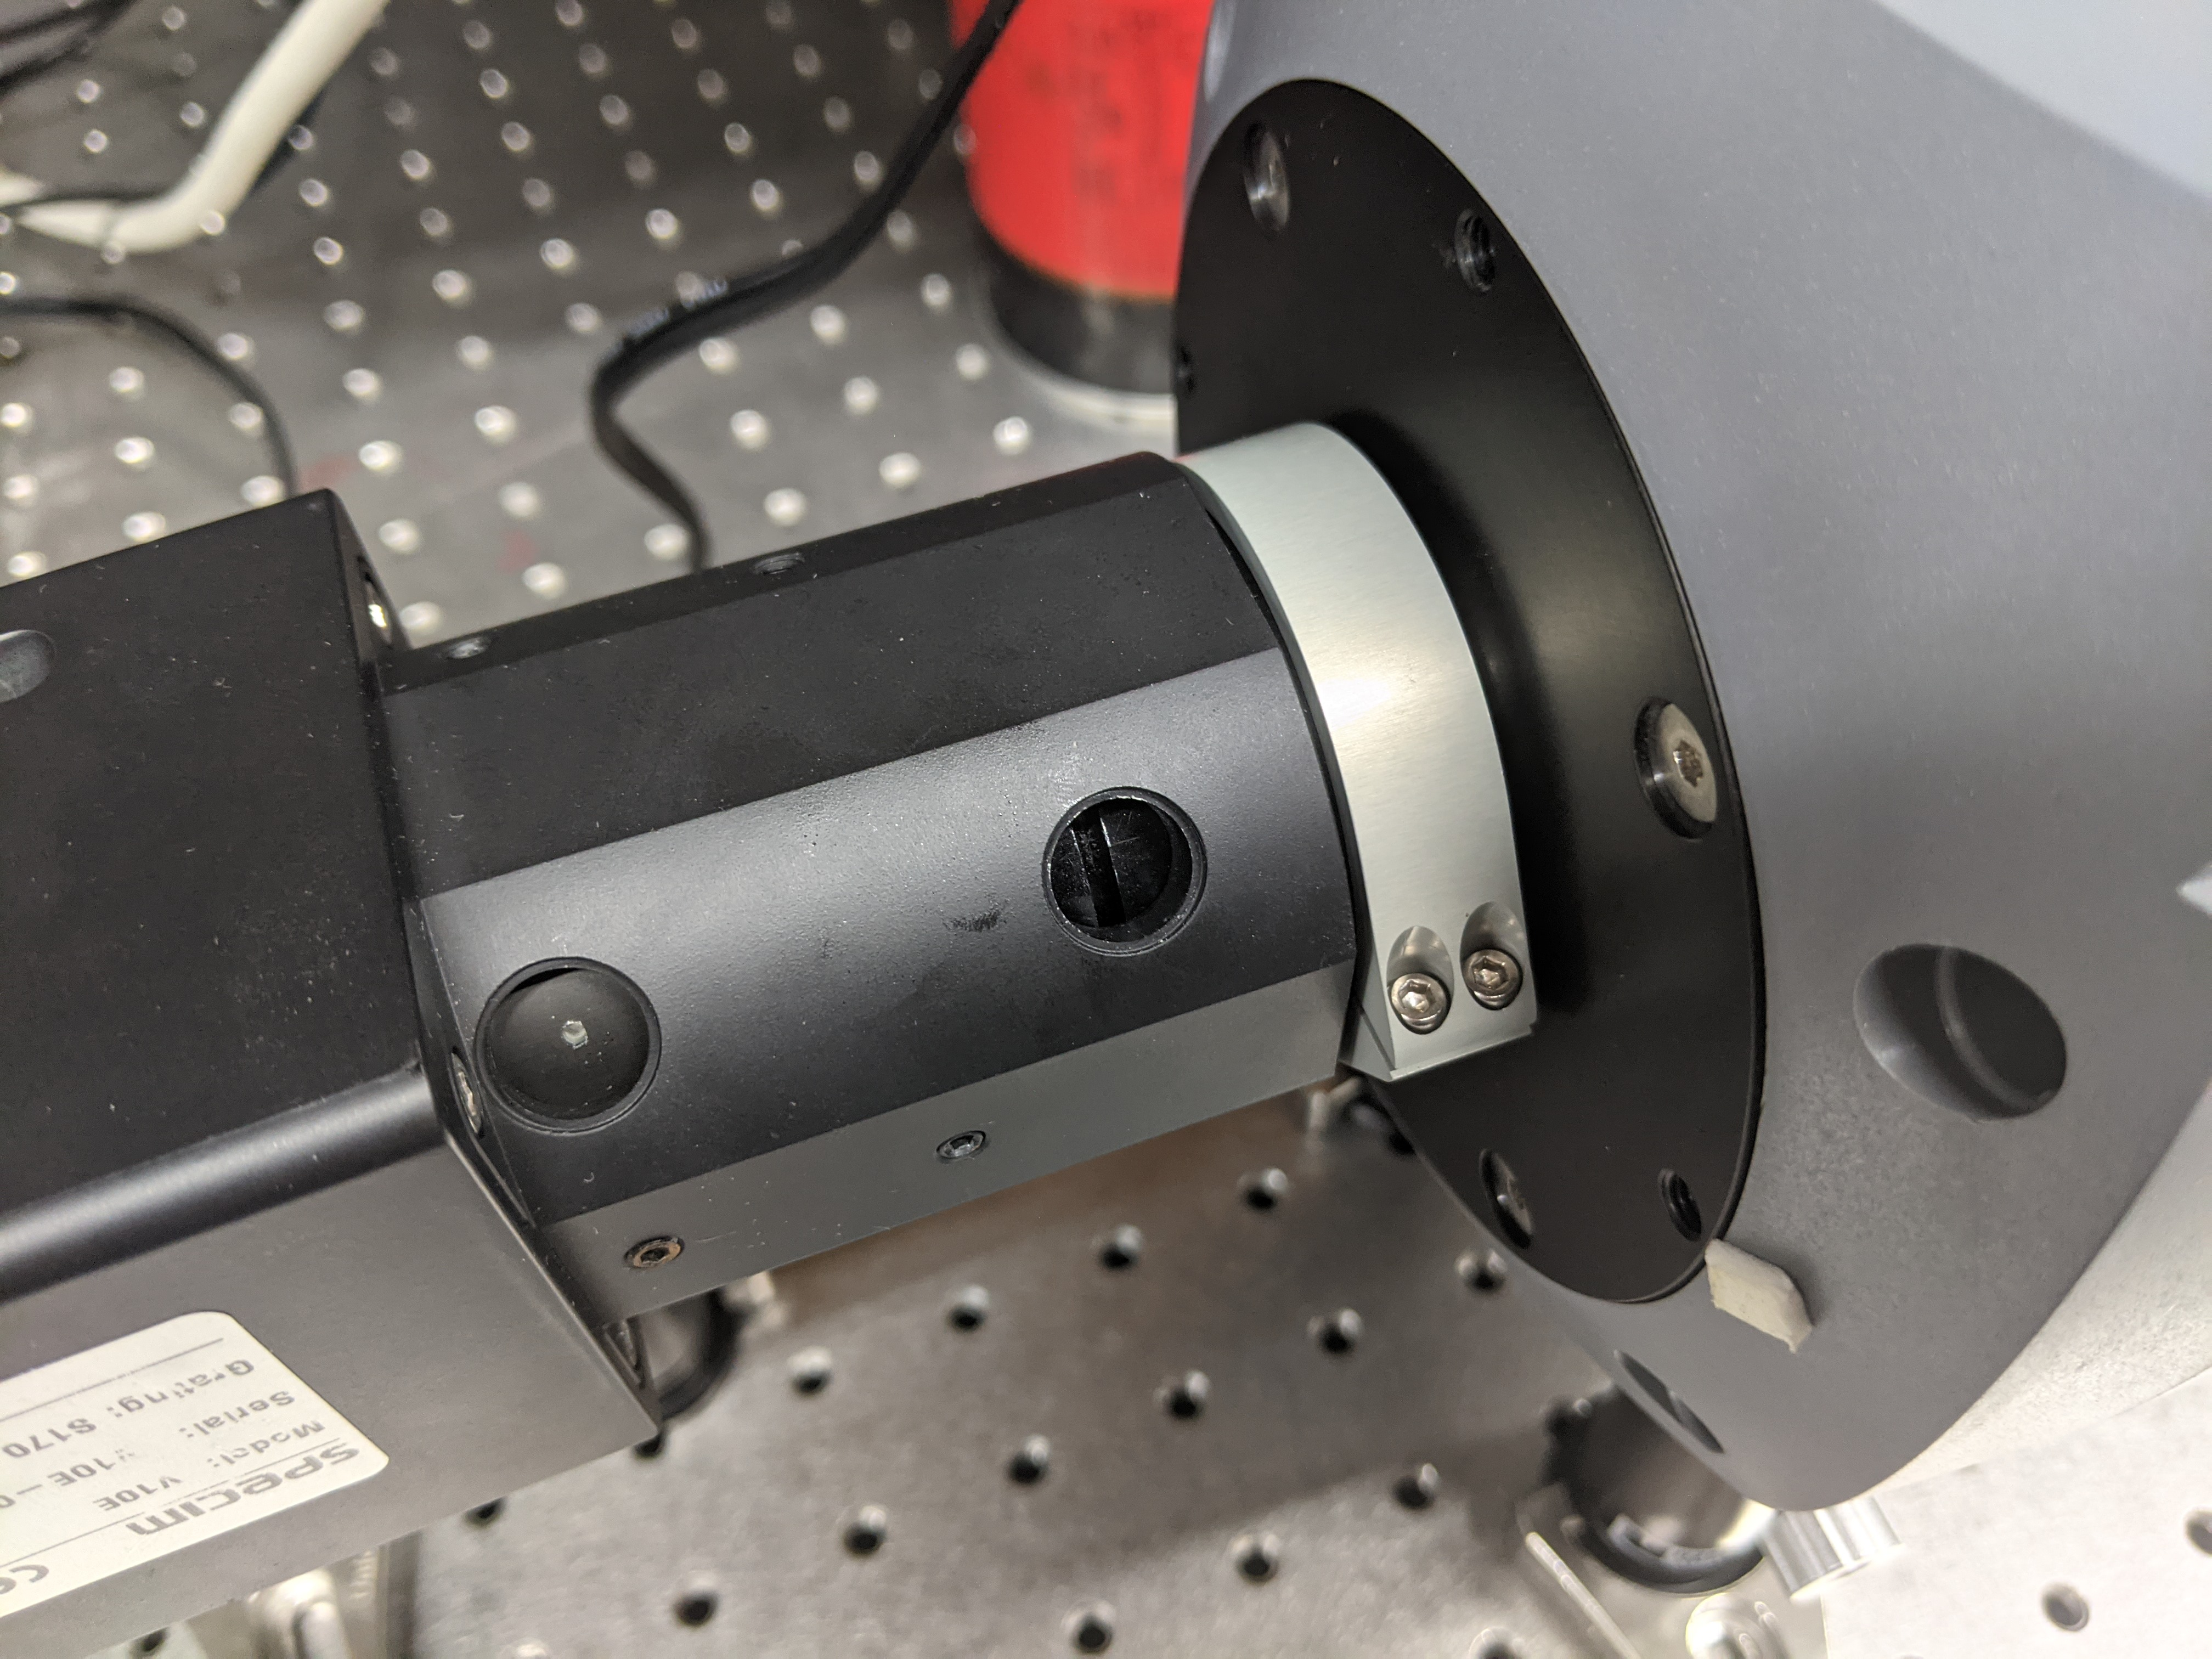
\includegraphics[width=0.65\linewidth]{PXL_20210507_105656554.jpg}
        \caption{Adjust the focusing element of V10E}
        \label{figure: specim bfp lens}
    \end{figure}

    \begin{figure}[t]
        \centering
        
\includegraphics[width=0.8\linewidth]{0423withoutobf.jpg}
        \caption{(on sensor image)Alingment between V10E and iXon}
        \label{figure: align v10e and ixon}
    \end{figure}

    \subsubsection{對焦}
    在巨觀的尺度,可以使用一個Specim 原廠所提供的圖樣(圖\ref{figure: focus pattern})來卻任物鏡的對焦。由於我們無法單純從iXon CCD上的影像判斷目前所觀測的位置,可以先把該圖案放在欲觀測的位置上,
    如圖所示,當線光譜儀觀測該圖案的不同位置時,可以明顯在CCD上看到不同的畫面。(圖\ref{figure: focus})

    觀測物經過物鏡成像後,僅有該像的中間一條細線範圍,能夠進入線光譜儀的入射狹縫,在進入線光譜儀後,該細線上的每一個點,
    會被展開成一光譜,成現在CCD的x軸上。因此,當物鏡準確對焦在這個圖案的正中間時,畫面上所呈現的應該是黑白相間的斑馬紋路,每條紋路的寬度均等,長度與照明光源的光譜有關。而條紋的邊緣應非常銳利,且黑色條紋極細。

    \begin{figure}[t]
        \centering
        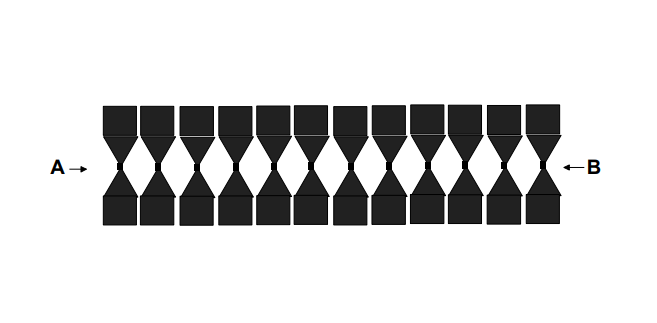
\includegraphics[width=0.8\linewidth]{focusPatern.png}
        \caption{The pattern for checking focus\cite{tn}}
        \label{figure: focus pattern}
    \end{figure}
    \begin{figure}[t]
        \centering
        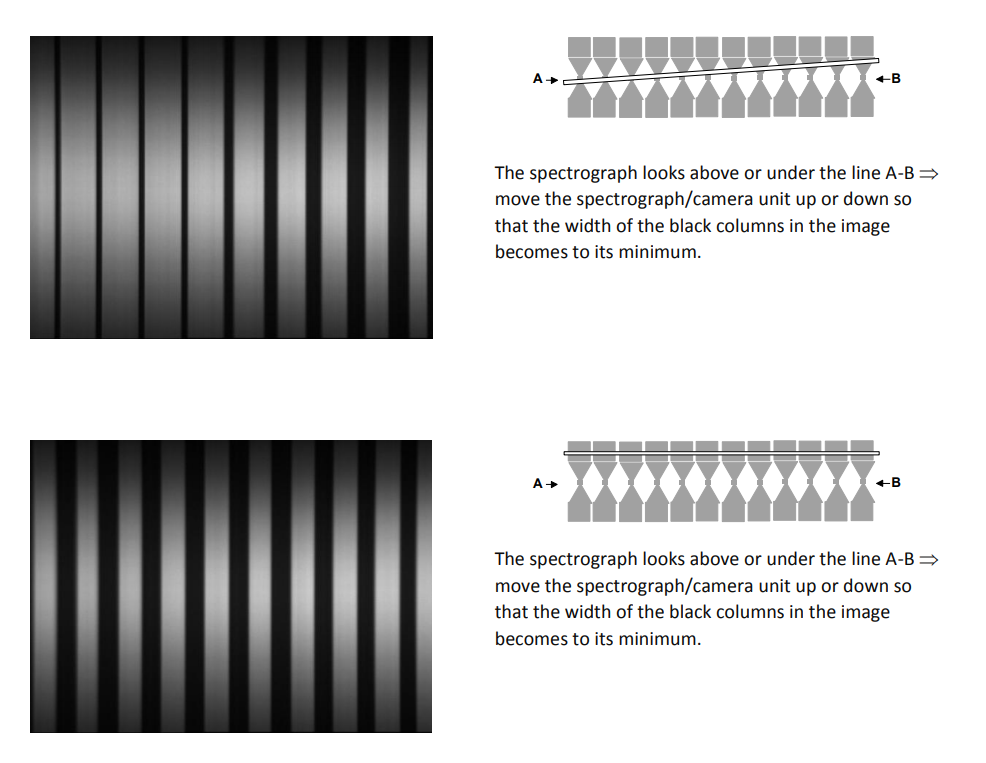
\includegraphics[width=0.6\linewidth]{errorOfFocus.png}
        \caption{(On sensor image)Possible error of focusing. \cite{tn}}
        \label{figure: focus}
    \end{figure}

    \subsection{Order Blocking Filter}
    由於Specim V10E的前玉為一狹縫,光線進入後,理應會發生單狹縫干涉,產生二階影像(Second order image),因此Specim系統中視時尚須搭配一個
    二階濾鏡(Order Blocking Filer),根據原廠的說明書,該濾鏡可以C-Mount安裝,或是直接黏貼在影像感測器上,不論以何種方式安裝,
    皆須盡量靠近影像感測器,實務上與影像感測器不宜超過6mm的距離\cite{manual}。
    \begin{figure}[t]
        \centering
        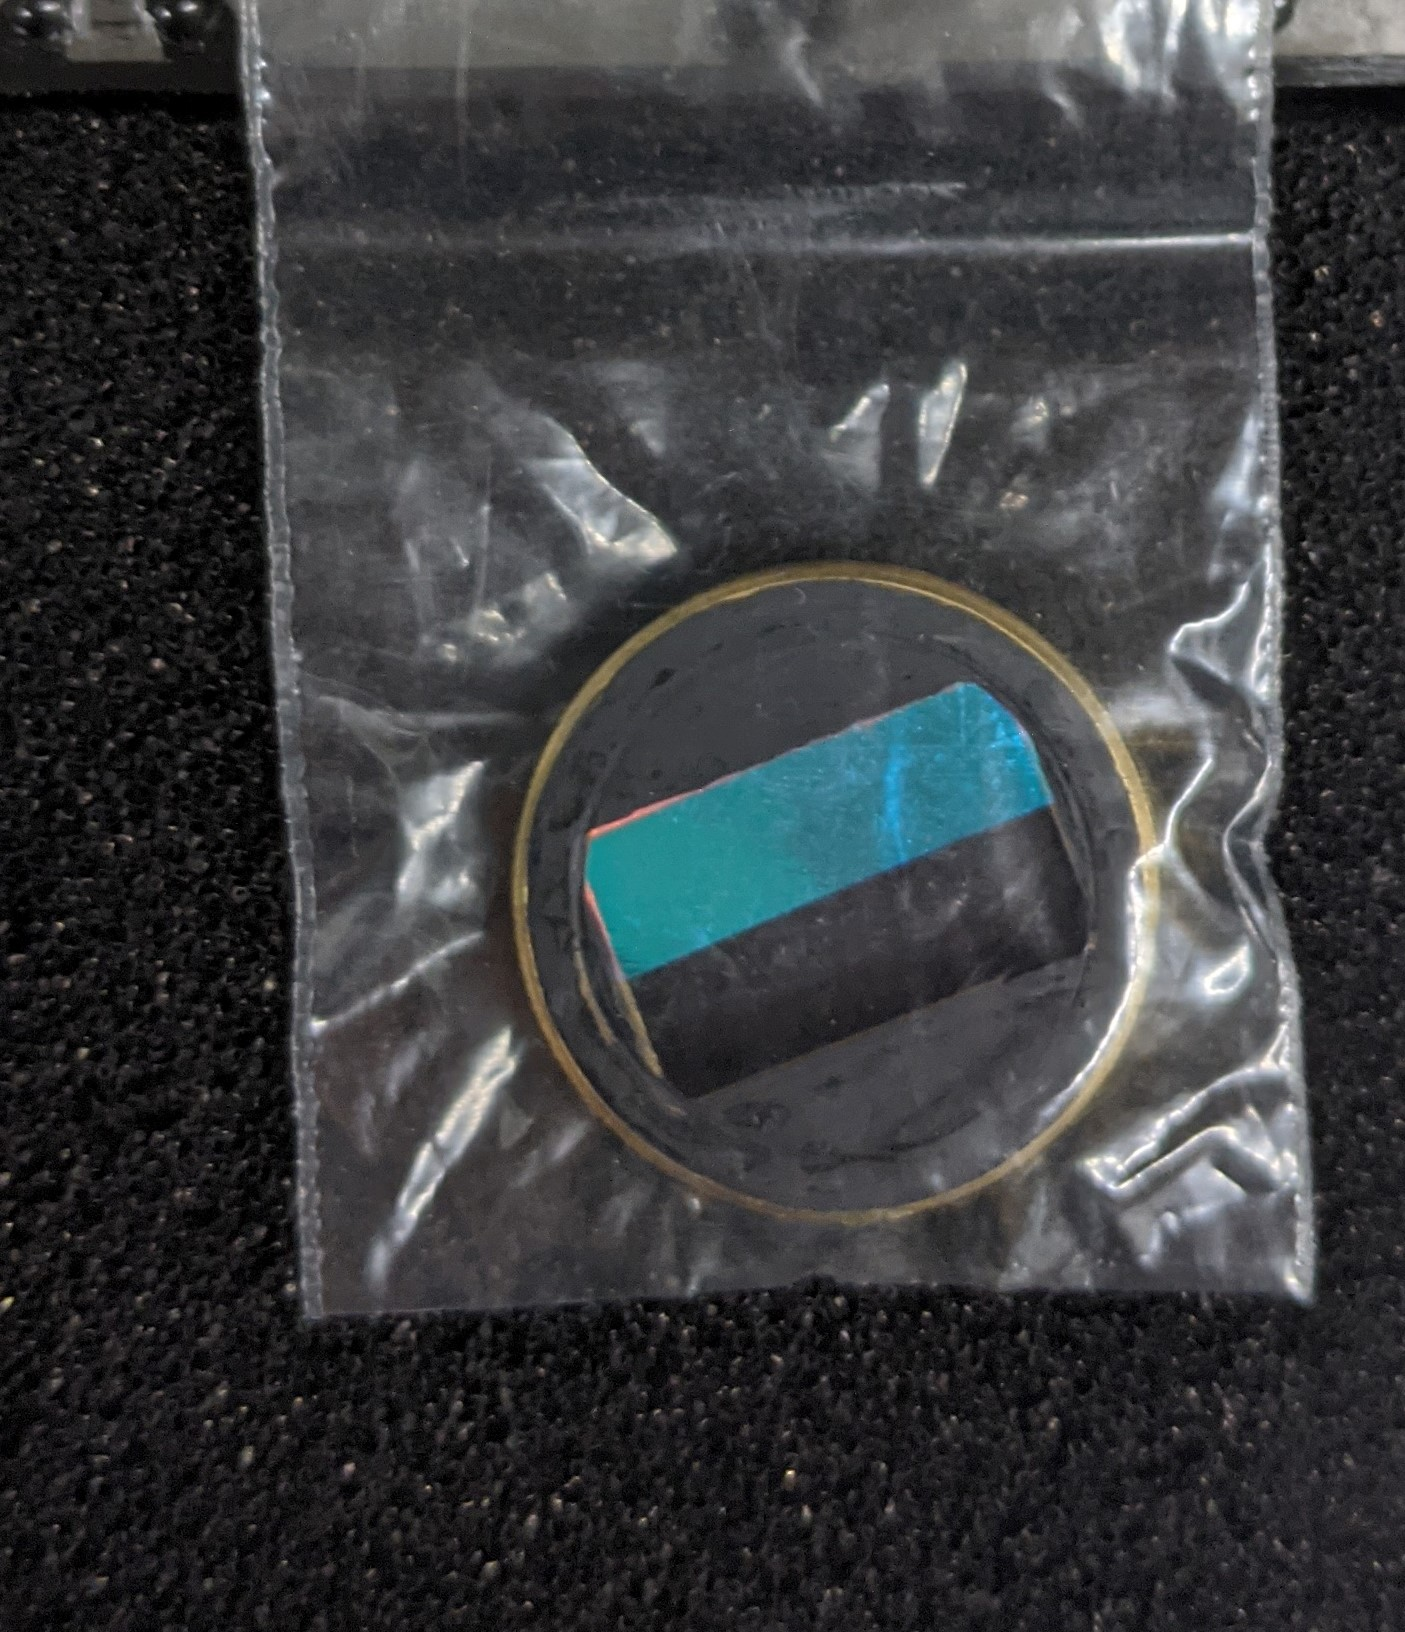
\includegraphics[width=0.5\linewidth]{PXL_20210723_094341395.jpg}
        \caption{The order blocking filter.}
        \label{figure: obf}
    \end{figure}
    觀察該濾鏡的外觀,可發現其阻擋二階干涉影像的方式,應該就是在鏡面上二階影像出現的位置度上塗層進行濾波。由於我們的系統上,不宜將濾鏡直接黏貼在昂貴的iXon EMCCD上,
    原本希望以C-mount方式安裝,但可行的安裝位置與影像感測器的距離都會超過6mm,就算克制專用的c-mount轉接環,仍至少會有約9.55mm左右的距離,我們擔心這樣反而會造成該濾鏡阻擋到原初的一階影像,
    因此最後決定先不安裝該濾鏡,待過後再來檢視二階影像的影響。事實上,在本系統的往後開發過程中,皆沒有在任何影像中看到二階干涉的影響,
    不過這是由於我們未曾使用超過30ms的曝光時間,在更長的曝光時間下,二階干涉是否會造成影響,值得後人加以深究。

    \section{第一階段: 軟體}
    \subsection{三維影像的建立}
    本系統所採用的線掃描 (Line scan or Push-broom) 影像原理,
    可以圖\ref{figure: lineScan}來說明。首先,系統中包含一個簡單的光學顯微鏡,
    能將樣品的像成在一部線光譜儀的入射狹縫上 ( 圖中的 input 
    slit),線光譜儀會同時對狹縫上的每個位置進行光譜量測 ( 圖中
    的 dispersion 示意 ),並在影像感測器上形成一個二維影像 ( 圖
    中 on sensor image),其包含了樣品掃描線上 512 個不同 Y 位
    置的光譜。接著只要再對樣品進行 X 方向的移動掃描,就能將各
    處單線的光譜影像組合成一張完整的高光譜影像 (Hyperspectral 
    image)。

    \begin{figure}[t]
        \centering
        \includegraphics[width=0.5\linewidth]{hsi_from_object_to_cube.jpg}
        \caption{線掃描的原理}
        \label{figure: lineScan}
    \end{figure}

    本系統在拍攝時,實際上從iXon EMCCD上擷取的On sensor image,如圖\ref{figure: linespectrum}所示,其縱軸與分光儀的狹縫同方向,因此也是代表樣品的空間縱軸,
    至於影像的橫軸刻度,則是代表不同波長。換句話說,在這張影像的每一個y位置,都有一條光譜線,在iXon EMCCD 512$\times$512像素的設定下,代表每一張on senson image
    上都有512個不同位置的光譜線。圖\ref{figure: linespectrum}是10x物鏡下,拍攝小型網格圖樣的影像,因此可以看見途中的亮帶與暗帶交錯。

    \begin{figure}[t]
        \centering
        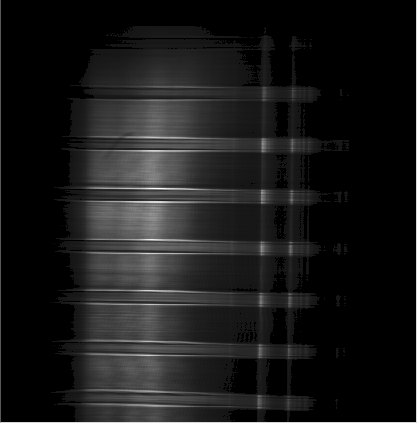
\includegraphics[width=0.5\linewidth]{lineSpectrum1213LDLS.png}
        \caption{網格的線掃描影像}
        \label{figure: linespectrum}
    \end{figure}

    實際上進行掃描時,只要在樣品上不同位置的掃描線擷取影像,就能得知樣品上每個位置的光譜資訊。每張線掃描影像皆是512$\times$512像素的二維影像,
    在掃描後,會得到數張這樣的二維影像,疊合後成為一張三維的影像,在程式中,是以三維的矩陣形式處裡。一開始所疊合而成的三維影像,其x,y,z軸分別為波長、樣品y、樣品x軸,
    與實際的樣品空間座標有出入,因此必須將矩陣的x與z軸調換(transpose),才能產生出一個與樣品空間相同的影像。該影像即是由512張(由於on sensor image在波長方向有512個pixel)各個波長下的樣品二維影像所組成。

    \subsection{影像儲存}
    掃描完成後的三維矩陣,我們將其儲存為TIFF影像格式。TIFF全名維Tagged Image File Format,顧名思義,其檔案中能儲存影像與描述影像的各式標籤(Tag)。
    除此之外,Tiff格式支援儲存多個的影像在一個檔案中,故我們能將三維矩陣的每一層二維影像,都儲存在同一個檔案中。

    Tiff檔案大致可分為兩部分,前半部分儲存的是檔案中每一張影像的標籤,描述了各式的影像資料,包括公版的影像資料標籤,如影像的像素數與位元等,也包括了我們自行加入的其他影像資料標籤,
    如每一層二維影像所在的波長,即是以一個一維陣列的方式儲存維一個自定義的影像資料標籤。

    檔案的後半部分,才是各張影像的實際資料。在我們的系統中,每個檔案一慮都會包含512張不同波長下的影像,這些影像也各都會有自己的一組影像資料標籤,這512組影像資料標籤也是都儲存在前半部分。

    我們使用實驗室過去留下的公版tiff labview library來進行影像檔案的儲存與其中影像資料標籤的管理,在開發初期遇到該library內資料寫入檔案時,端序(byte order)不一致的問題,有些資料是以大端序(big endian),
    寫入,有些是以小端序(little endian)寫入,為了配合實驗室Analyser軟體,我們最後一慮皆使用小段序寫入資料。

    \subsection{座標校正}
    \subsubsection{空間x軸校正}
    空間x軸的校正,旨在得知影像上x方向對應到的實際尺寸,與每一個像素在實際空間所在的位置。由於本系統是沿著x方向進行掃描,在電動載台移動到指定位置後,才擷取一張線掃描影像,由於電動載台的位置是已知的,因此也能夠知道自然每個x方向像素所在的實際位置。
    不過在設定電動載台移動距離時,還須注意到掃描線在樣品上實際的寬度,雖然很微小,但仍是存在。依據Specim的說明書,樣品上掃描線的實際寬度,可以
    \begin{equation*}
        W=\frac{W_s\times D}{f}
    \end{equation*}
    來計算,其中$W_s$是狹縫的寬度,$D$是樣品與鏡頭的距離,$f$則是物鏡的焦距。如果電動載台掃描時移動的距離比該寬度還小,實際上就代表每條掃描線之間有重疊,因此在軟體設計上會提示使用者依據此式算是計算出的建議掃描步進。
    $W_s$、$D$、$f$則分別以知名儲存在ini檔案中,以協助軟體計算。
    \subsubsection{空間y軸校正}
    與尚述相同,空間y軸的校正,旨在得知影像上y方向對應到的實際尺寸,與每一個y軸像素於實際空間中所在的位置。實務上要校正y軸,就是要得知入射狹縫上的像在樣品上的實際尺寸。由於狹縫上的像已可視為是一維的影像,所以也可說是要得知狹縫高實際上在樣品上所應的長度。
    在本階段的巨觀尺度下,可以拍攝已知高度與刻度的圖樣,如下圖\ref{figure: self pattern},的on sensor image,並在其上計算y方向亮暗帶交錯的次數,即可得知狹縫的y視野,在後面微觀的系統下,
    我們以已知方格大小的銅網螢光片來計算,也可得知影像y軸的實際尺寸,並將其儲存在ini檔的項目中。
    \begin{figure}[t]
        \centering
        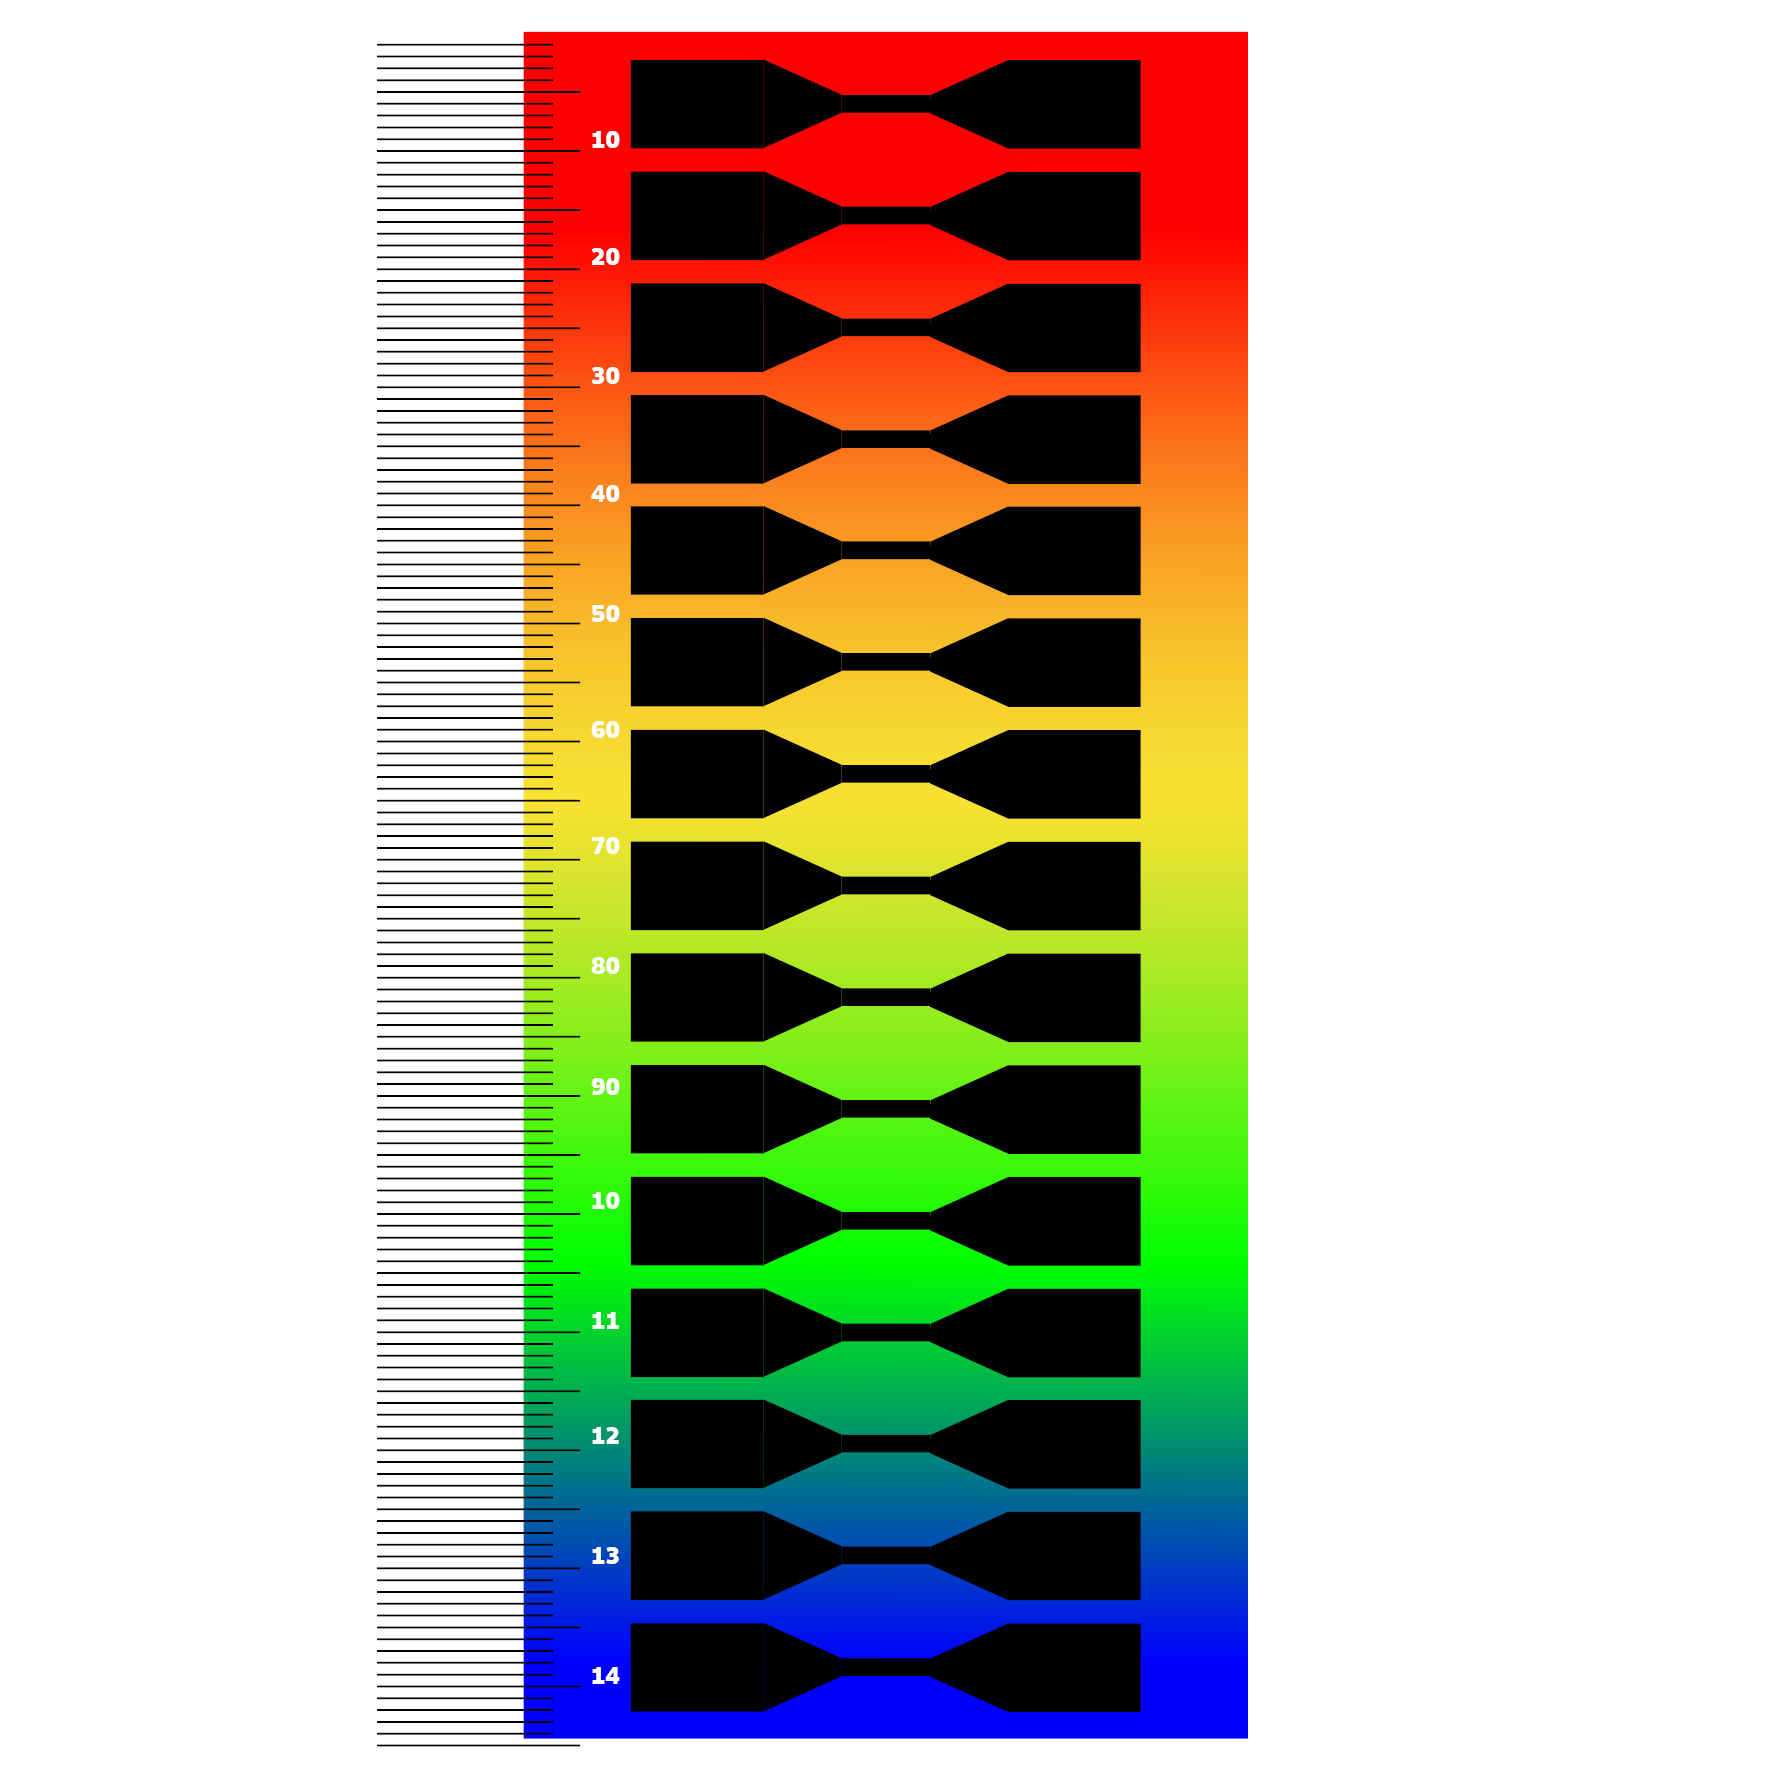
\includegraphics[width=0.4\linewidth]{patternColor.jpg}
        \caption{A self-designed pattern for focusing and calibration.}
        \label{figure: self pattern}
    \end{figure}
    \subsubsection{波長軸(z)校正}
    所謂波長軸的校正,就是要知道on sensor image上每個x軸像素所代表的波長,或說是最終三維影像資料中,每一層二維影像所在的波長。在本階段巨觀系統硬體下,校正方式是將
    標準光源(cal-2000)自物鏡前方直接打入,並在iXon隨附的Solis軟體中得出on snesor image在x方向的平均line profile,
    接著精確讀出x方向上每個訊號強度波峰所在的x像素,並與標準光源的已知光譜以線性回歸線推出進行減量線,其斜率與截距儲存在ini檔的項目中,軟體即會自動計算並調整螢幕上所顯示的波長。
    在接下來微觀系統的校正,方法亦相同,但由於微觀系統採用內部照明的方式,標準光源以光纖方式進入系統,此時僅需在樣品處放置一個銀鏡,即可量測標準光源離開物鏡打到銀鏡後的反射光譜。
    
    \begin{figure}[t]
        \centering
        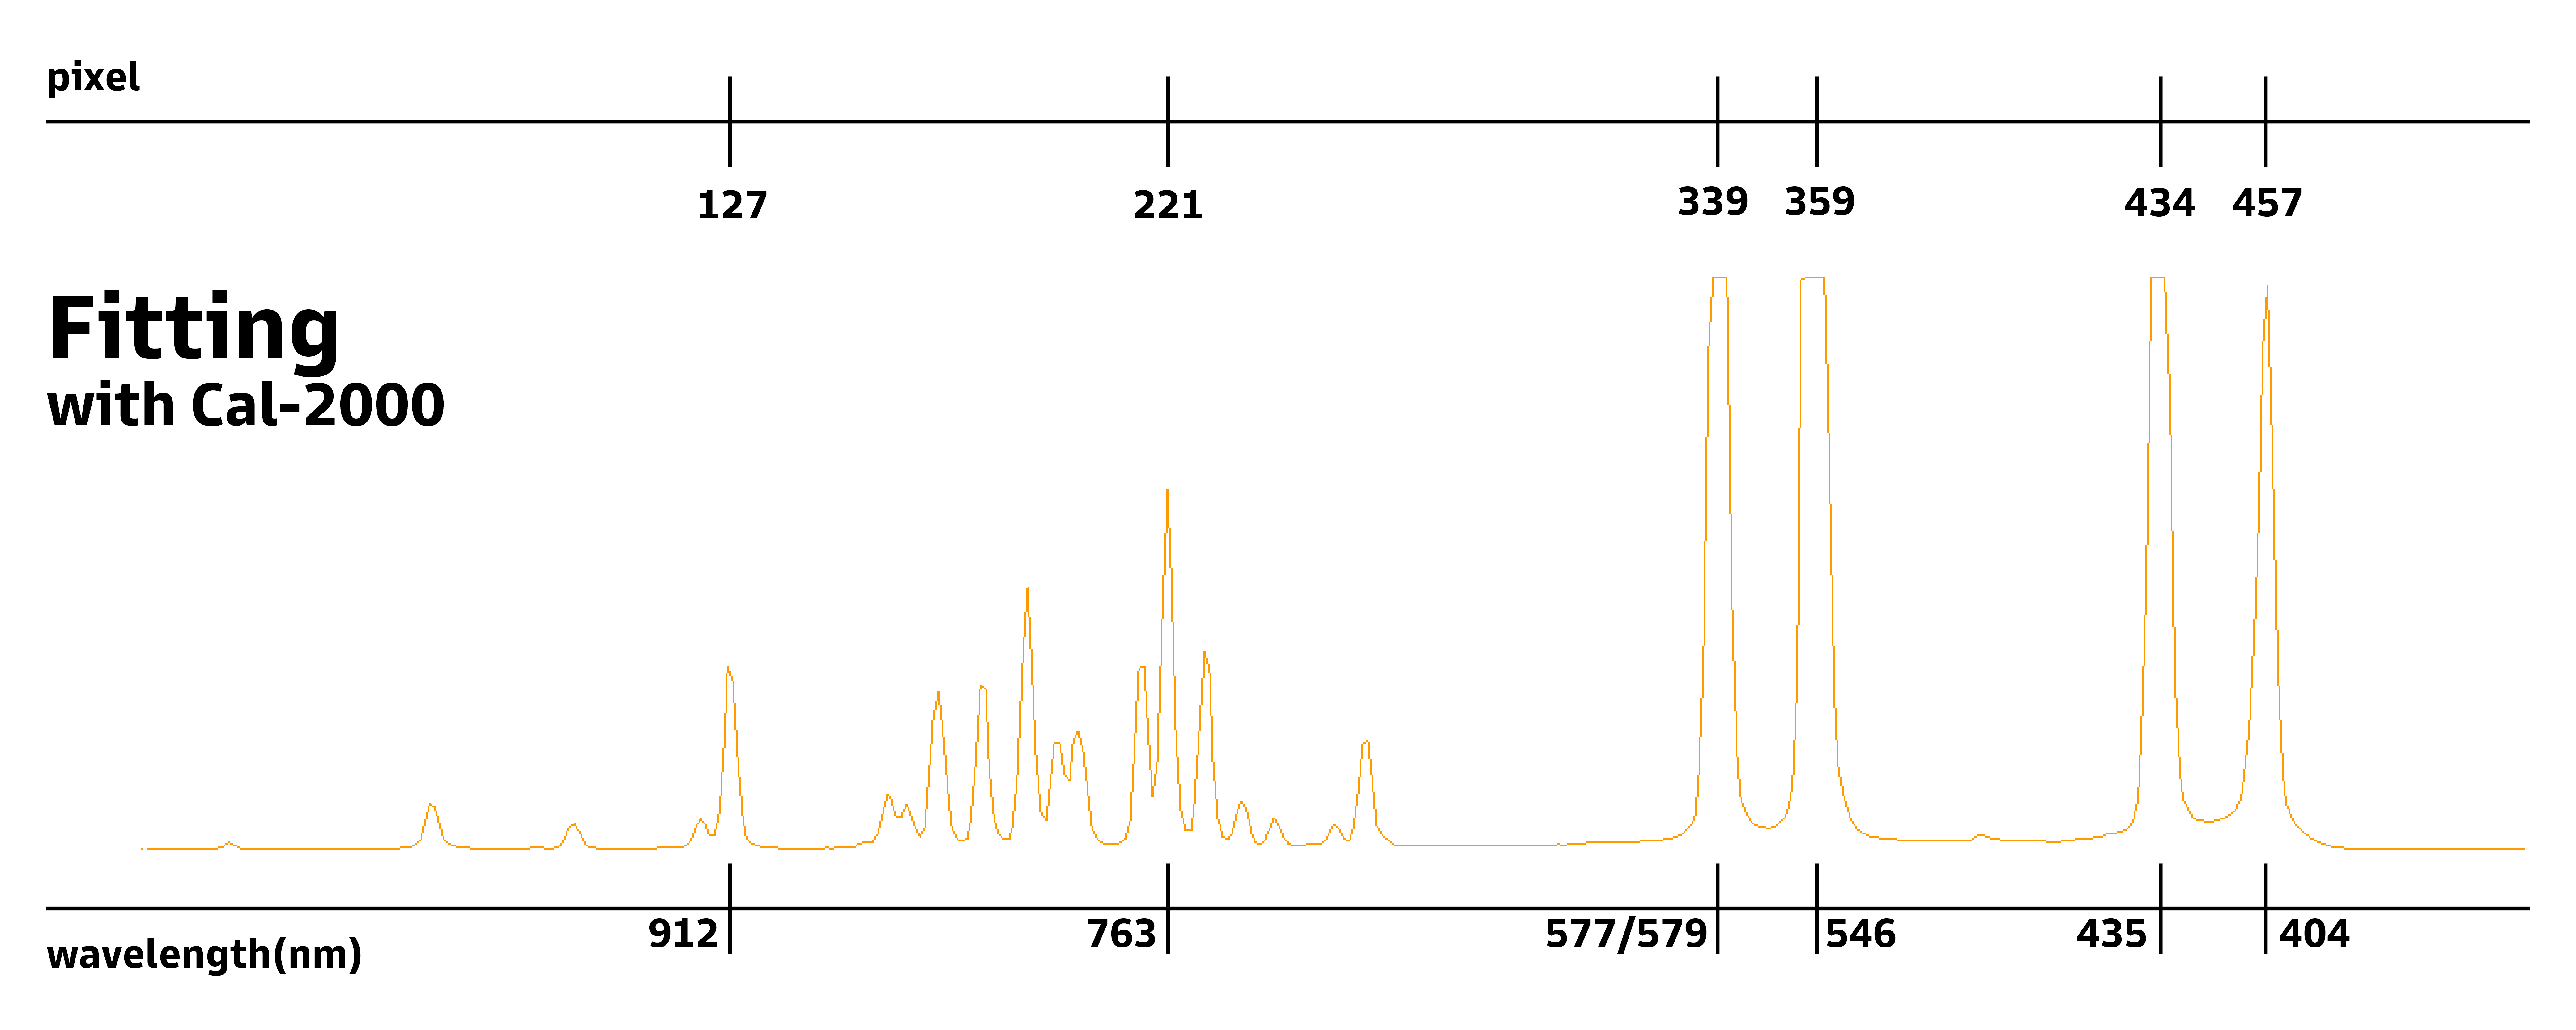
\includegraphics[width=\linewidth]{fitting.jpg}
        \caption{以cal-2000進行校正}
        \label{figure: fitting}
    \end{figure}
    \begin{figure}[t]
        \centering
        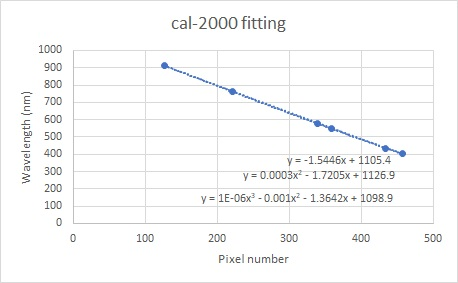
\includegraphics[width=\linewidth]{cal-2000fitting.jpg}
        \caption[]{波長軸校正減量線\protect\footnotemark}
        \label{figure: fit curve}
    \end{figure}
    \footnotetext{請注意,校正時必須導出與本圖相似的負斜率減量線,若導出的減量線為正斜率,可以在Solis軟體中Acquisition setting設定flip image。}
    \section{第二階段: 硬體}
    第二階段的系統,主要目的在於將同樣的線掃描技術,應用於微觀尺度,硬體上的變更,首要就是將原本第一階段所採用的23mm camera lens,置換成一具簡單的光學顯微鏡。我們採用了Olympus 的10x顯微物鏡,
    並搭配15 cm的tube lens,將放大過後的樣品影像成在分光儀的入射狹縫上,至於分光儀與iXon影像感測器的設置,則沒有不同。

    除此之外,系統的照明方式也有改變。原初以外部照光的方式,對於所需照明範圍相對較小的顯微影像來說,會浪費較多光源,也不適合進行雷射螢光等觀測,
    因此將照明方式改為內部照明,系統上有兩個光纖collimator,能夠彼此切換。光源經過tube lens匯聚在物鏡的背焦面上,通過物鏡後變成平行光,以期照射在樣品上的光線最為均勻。

    裝設物鏡的鏡架,能夠上下移動以進行對焦,光源的tube lens也能微調位置。物鏡的tube lens雖然裝設在可調的鏡筒內,但不應任意移動。至於電動載臺的裝設與使用,則沒有不同。
    系統上另外再成像進入分光儀狹縫前,已一片半反射鏡將OM影像投至一臺Canon M2相機中,借助其APS-C尺寸的感光元件,能夠完整顯示出OM的視野,以幫助使用者尋找ROI。
    \begin{figure}
        \centering
        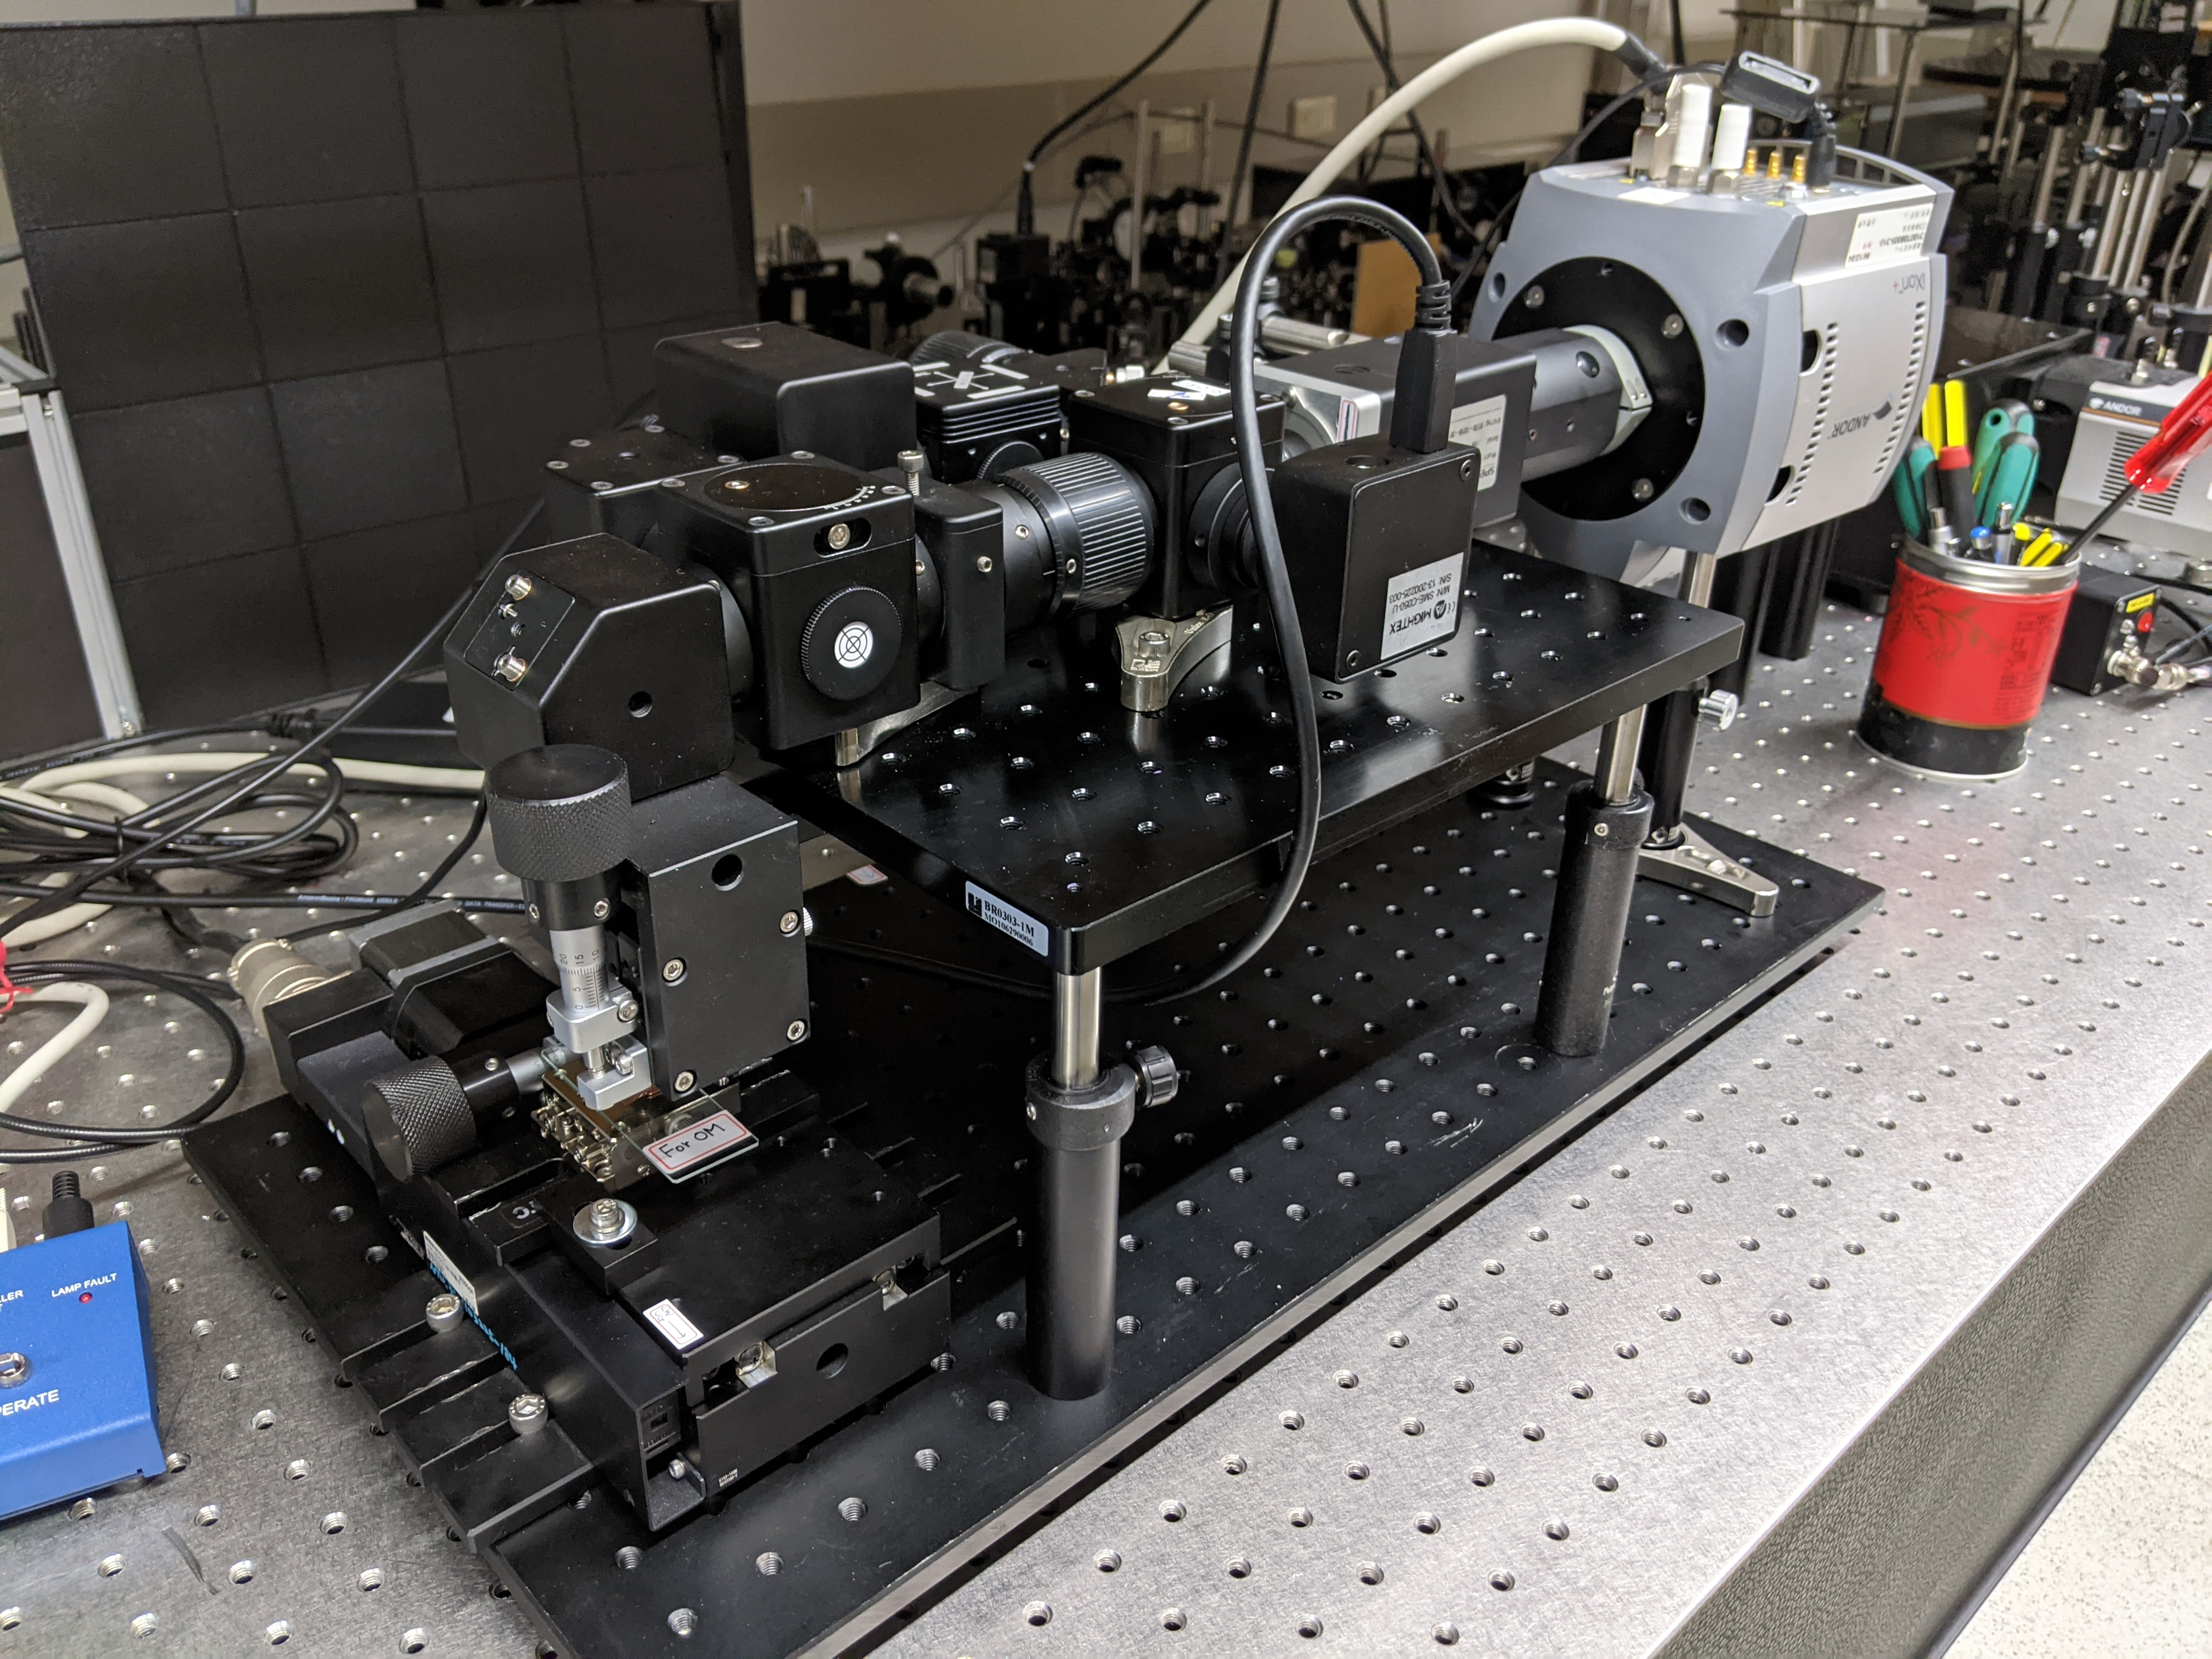
\includegraphics[width=\linewidth]{PXL_20210831_081957648.jpg}
        \caption{Micro system.}
    \end{figure}

    \subsection{Galvo}
    在最早的規劃中,第二階段的系統應該要從第一階段移動樣品的方式,改成以Galvo進行移動光源的方式掃描,但經過評估後,發現Galvo的運作方式並不適合線掃描系統。Galvo掃描的原理,是改變點光源照射在樣品上的位置,
    以一一對樣品上各個位置進行光譜量射。由於線掃描方式一次至少要將樣品上的整條掃描線完整照明,若以Galvo調動點光源的位置,則代表需要將光源在曝光時間內完整掃描一次樣品上的掃描線,並將掃描線上不同位置的像對應到狹縫上的不同位置。
    然後,這樣勢必代表仍必須以電動載台移動樣品,才能將樣品上不同位置的掃描線之影像成在固定位置的狹縫上,如此的作法與現階段以面光源照滿光學顯微鏡視野,並移動載台的方式,並無效率上的優勢,
    且以面光源照明尚有更方便使用者尋找ROI的優點。雖然以點光源方式理應可以相同的光源提供更強的照明,但在系統開發過程中亦沒有遇到照明強度不足的問題,因此就沿用第一階段以電動載台移動樣品的掃描方式。
    \subsection{照明}
    本系統現階段的照明設備,分別是高頻寬的Energetic LDLS與405 nm的DPSSL Laser,從兩個光纖collimator進入系統。照明光路的目標是希望能進樣擴大照明範圍,並使照明盡量均勻。
    然而在系統架設的初期,energetic的照明存在明顯的上下不均勻現象,如圖與圖的比較所示,圖是初期進行光陸校正時使用的HL-2000光源照明下的影像,可以看見將同樣的光纖接頭改接LDLS光源後,照明變得非常不均勻。
    且視野上下幾乎已經超出照明範圍。請這些都是在確認照明光路經過校正後的影像。
    \begin{figure}
        \centering
        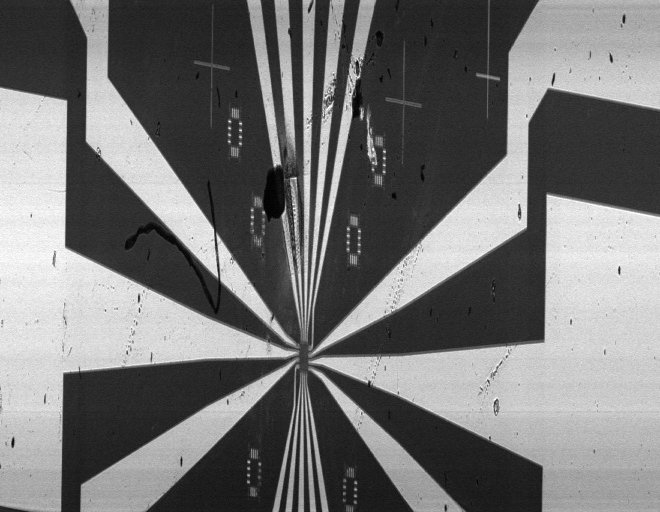
\includegraphics[width=0.5\linewidth]{0831focusForOmFullScanHL2000Scaled.jpg}
        \caption{HL-2000}
    \end{figure}
    \begin{figure}
        \centering
        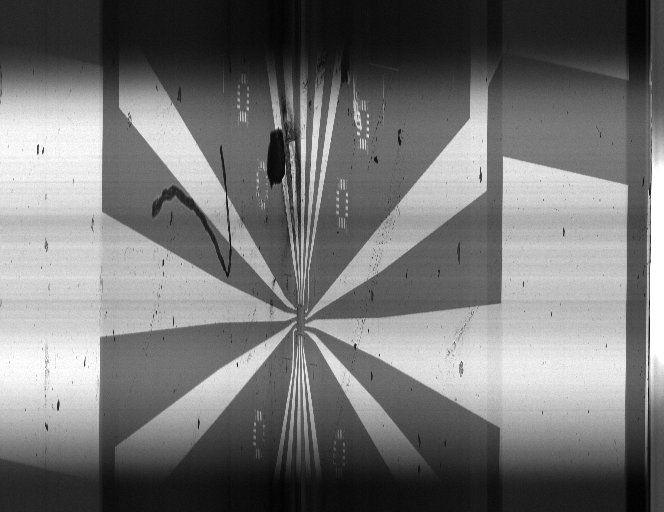
\includegraphics[width=0.5\linewidth]{0909Energetic.jpg}
        \caption{Energetic}
    \end{figure}
    為了改善照明的範圍,我們首先將原本使用的12.5cm tube lens換成現在所使用的15cm tube lens,希望能更集中使用成像中間較亮的部分,不過改善的效果有限,且系統上也沒有空間再裝設焦聚更長的透鏡。
    為了要進一步改善照明的均勻度,我決定嘗試調整LDLS光源系統內,光線進入光纖的Coupler,以及光線離開光纖,進入影像系統的Collimator。經過多次嘗試後,最終得出三種組態,可以藉此瞭解前述兩個組件對於照明的影響。
    \subsubsection{最高亮度、匯聚於背焦面} \label{section: illuOriginal}
    簡言之,平移調整光線進入光纖的Coupler,會決定LDLS的照明光譜中進入光纖的波段。該Coupler原先的狀態,是調整至照明亮度最高,也可視為是最寬的頻寬進入光纖的狀態。
    而光線離開光纖,進入照明系統的Collimator,即是一個可前後調整的透鏡,則會決定照明光源在影像系統內的何處匯聚。原先是調整至會剛好使照明光源正好匯聚在顯微物鏡背焦面的位置,使打在樣品上的光線為平行光。
    在這個設定下,掃描所得的影像如圖\ref{figure: brightest_on},可以看到影像上下明顯較暗,表示照明範圍還不夠大。從圖\ref{figure: om_brightest_on}的彩色OM影像可以看到,照明光源有類似色相差的情形出現,
    照明光源的影像不完整,且顏色也有分布偏移的情形。不過整體的照明尚算均勻,沒有明顯的干擾。
    \begin{figure}[t]
        \centering
        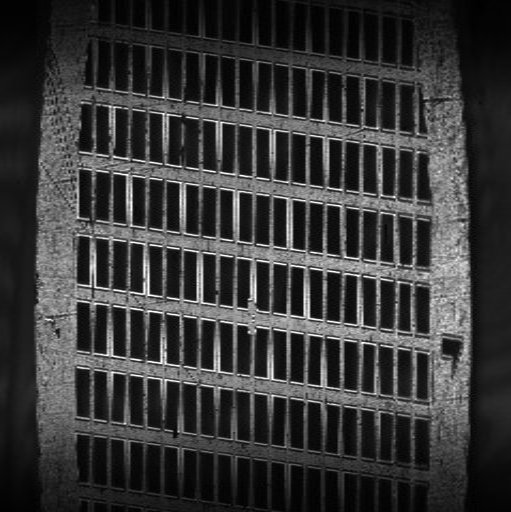
\includegraphics[width=0.5\linewidth]{on_brightest.jpg}
        \caption{Coupled at brightest, collimated on BFP.}
        \label{figure: brightest_on}
    \end{figure}
    \begin{figure}[t]
        \centering
        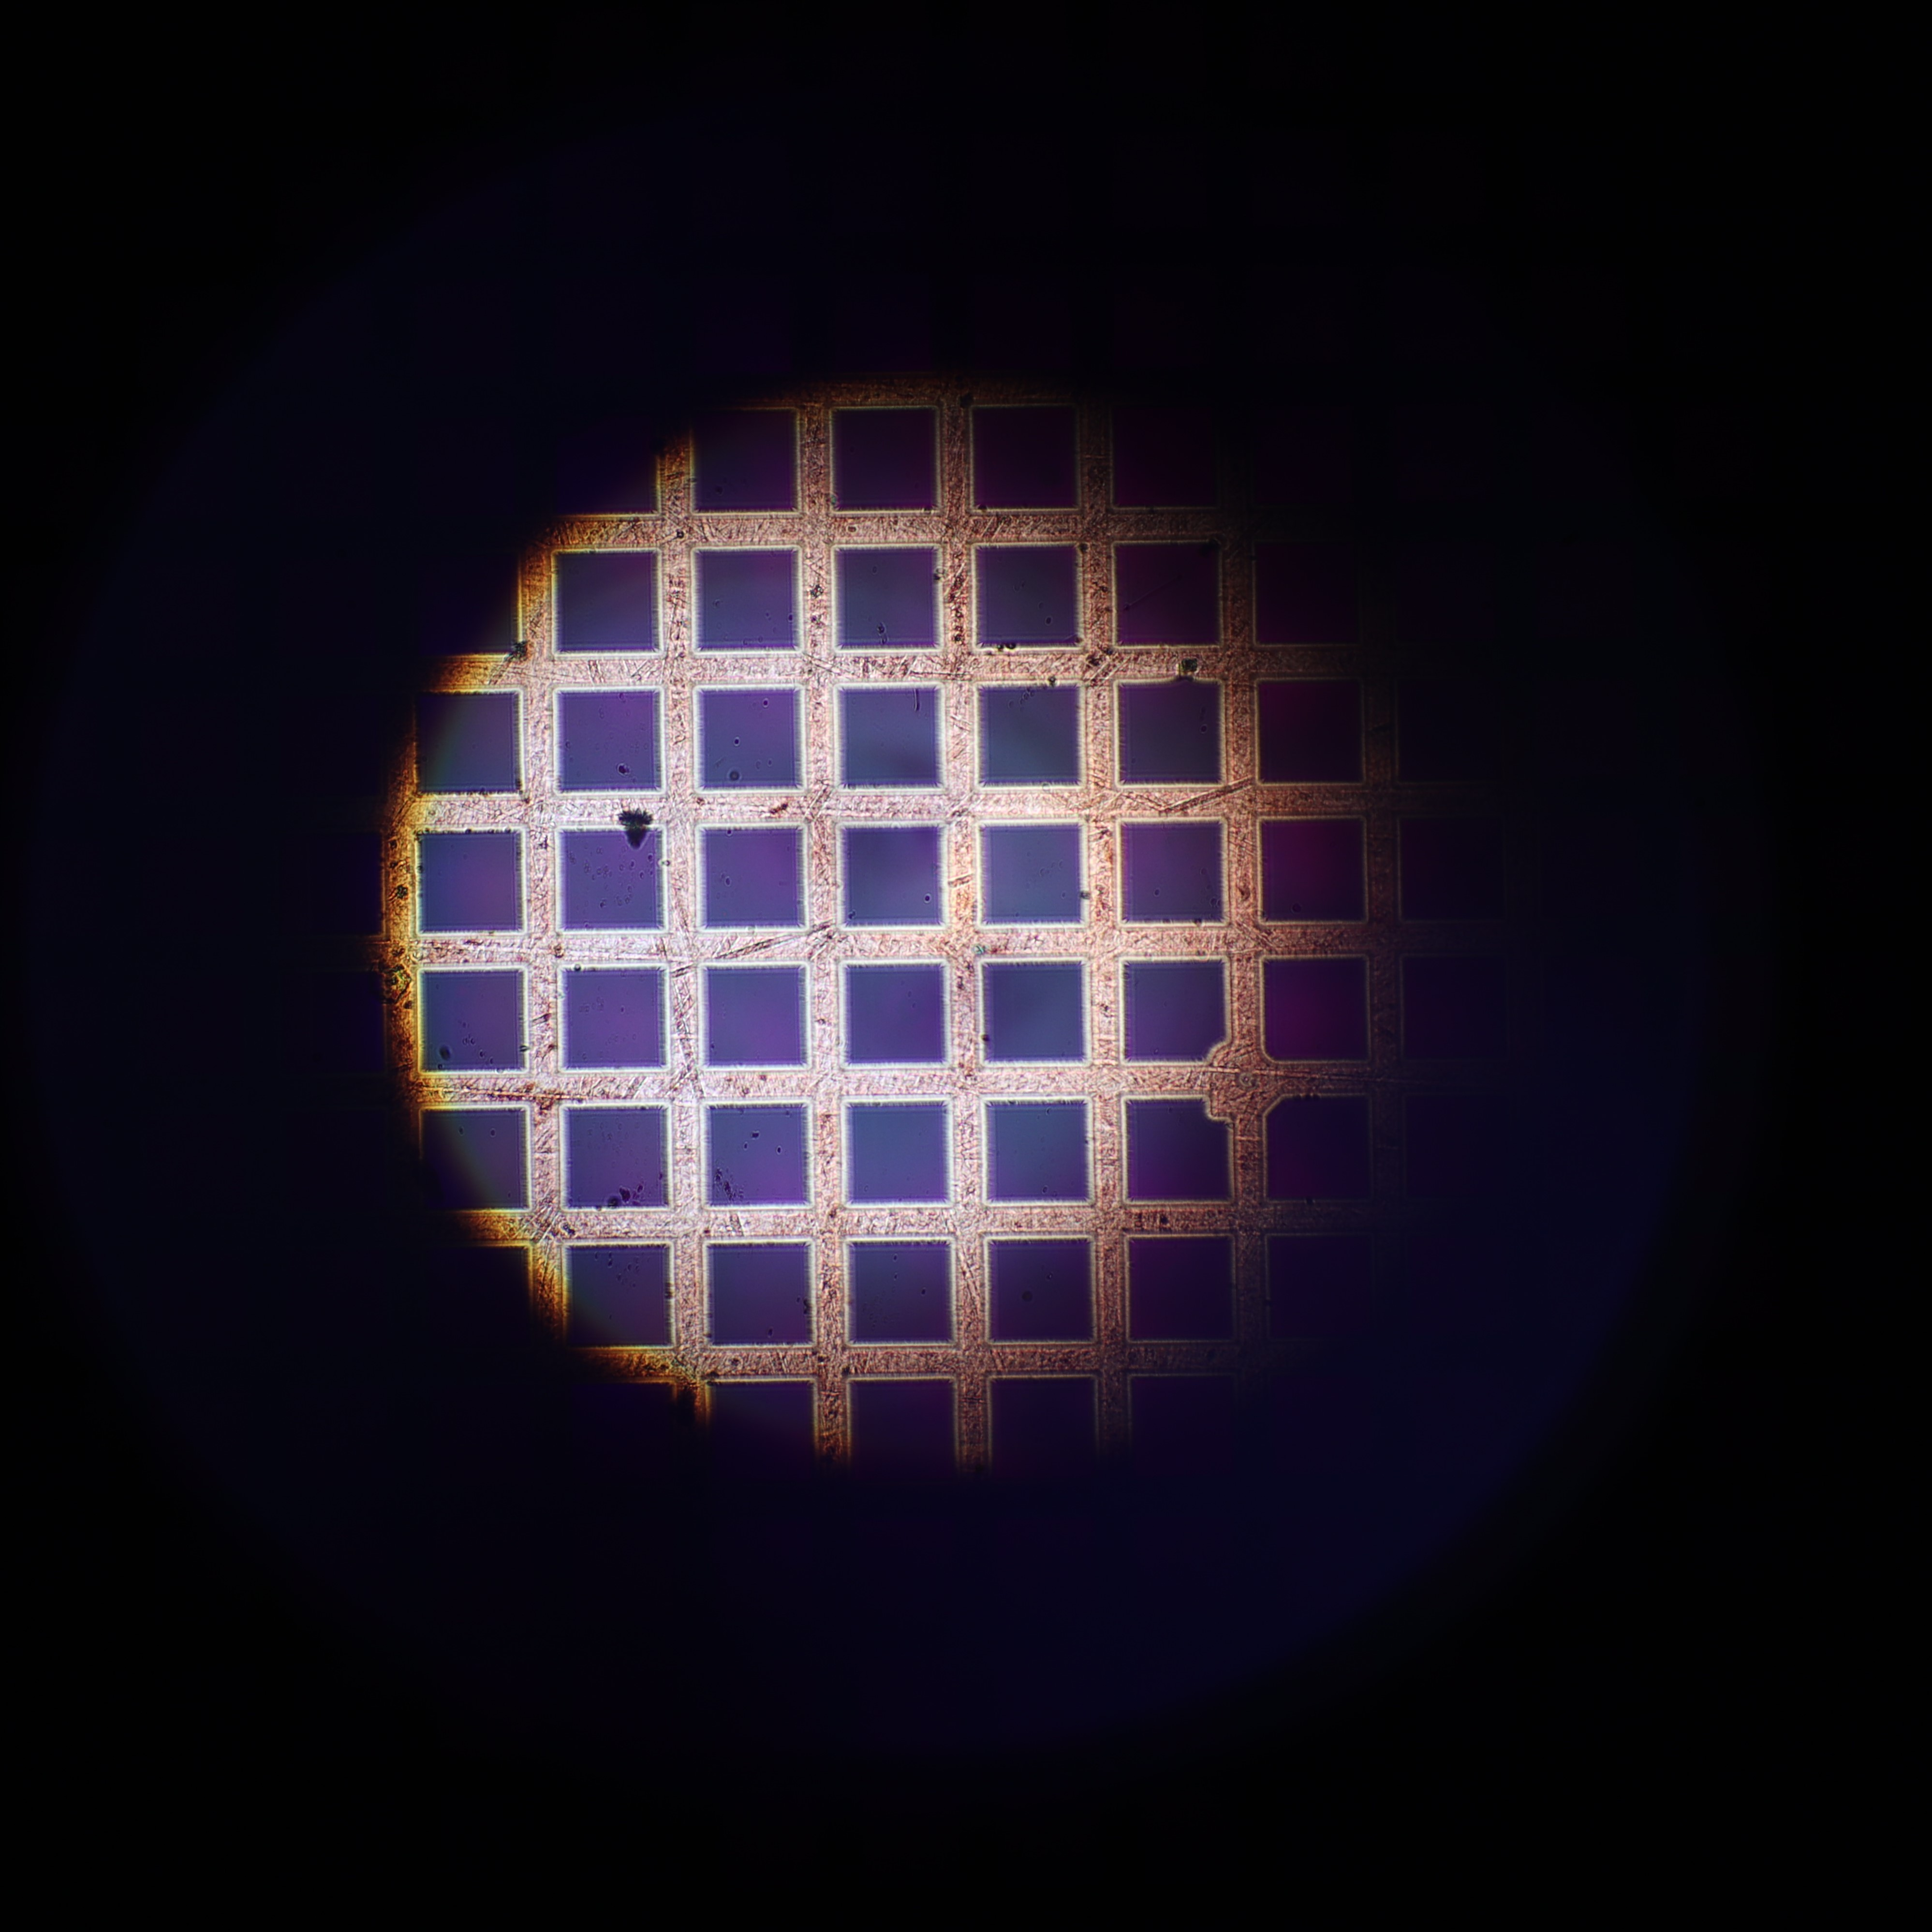
\includegraphics[width=0.5\linewidth]{om_on_brightest.JPG}
        \caption{OM: Coupled at brightest, collimated on BFP.}
        \label{figure: om_brightest_on}
    \end{figure}
    \subsubsection{最高亮度、不匯聚於背焦面}
    從前述的設定開始做調整,若將Collimator稍微調動,使光源不要匯聚在顯微物鏡的背焦面上,可以把照明的範圍再做擴大,並完整的照滿整個物鏡視野,如圖\ref{figure: brightest_off}、\ref{figure: om_brightest_off}所示,影像不再有上下明顯的暗帶。由於光線並未匯聚於物鏡的背焦面,打在樣品上的光線並非平行光,
    因此容易產生干擾的照明圖樣。以該螢光便樣品為例,由於螢光片半透明且具有厚度,不平行的光線穿過螢光片後,經反射後會產生不均勻的照明圖樣。
    \begin{figure}
        \centering
        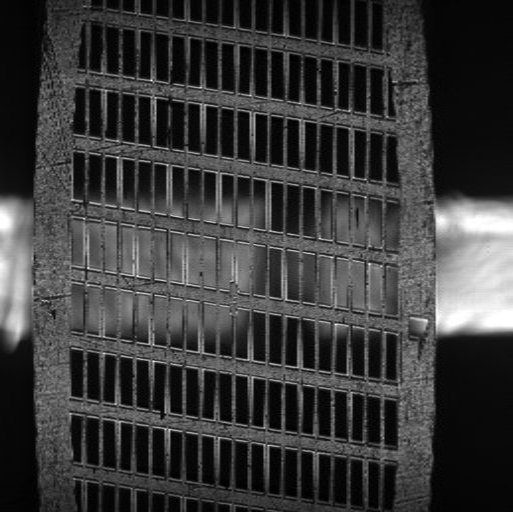
\includegraphics[width=0.5\linewidth]{off_brightest.jpg}
        \caption{Coupled at brighest, collimated off BFP.}
        \label{figure: brightest_off}
    \end{figure}
    \begin{figure}
        \centering
        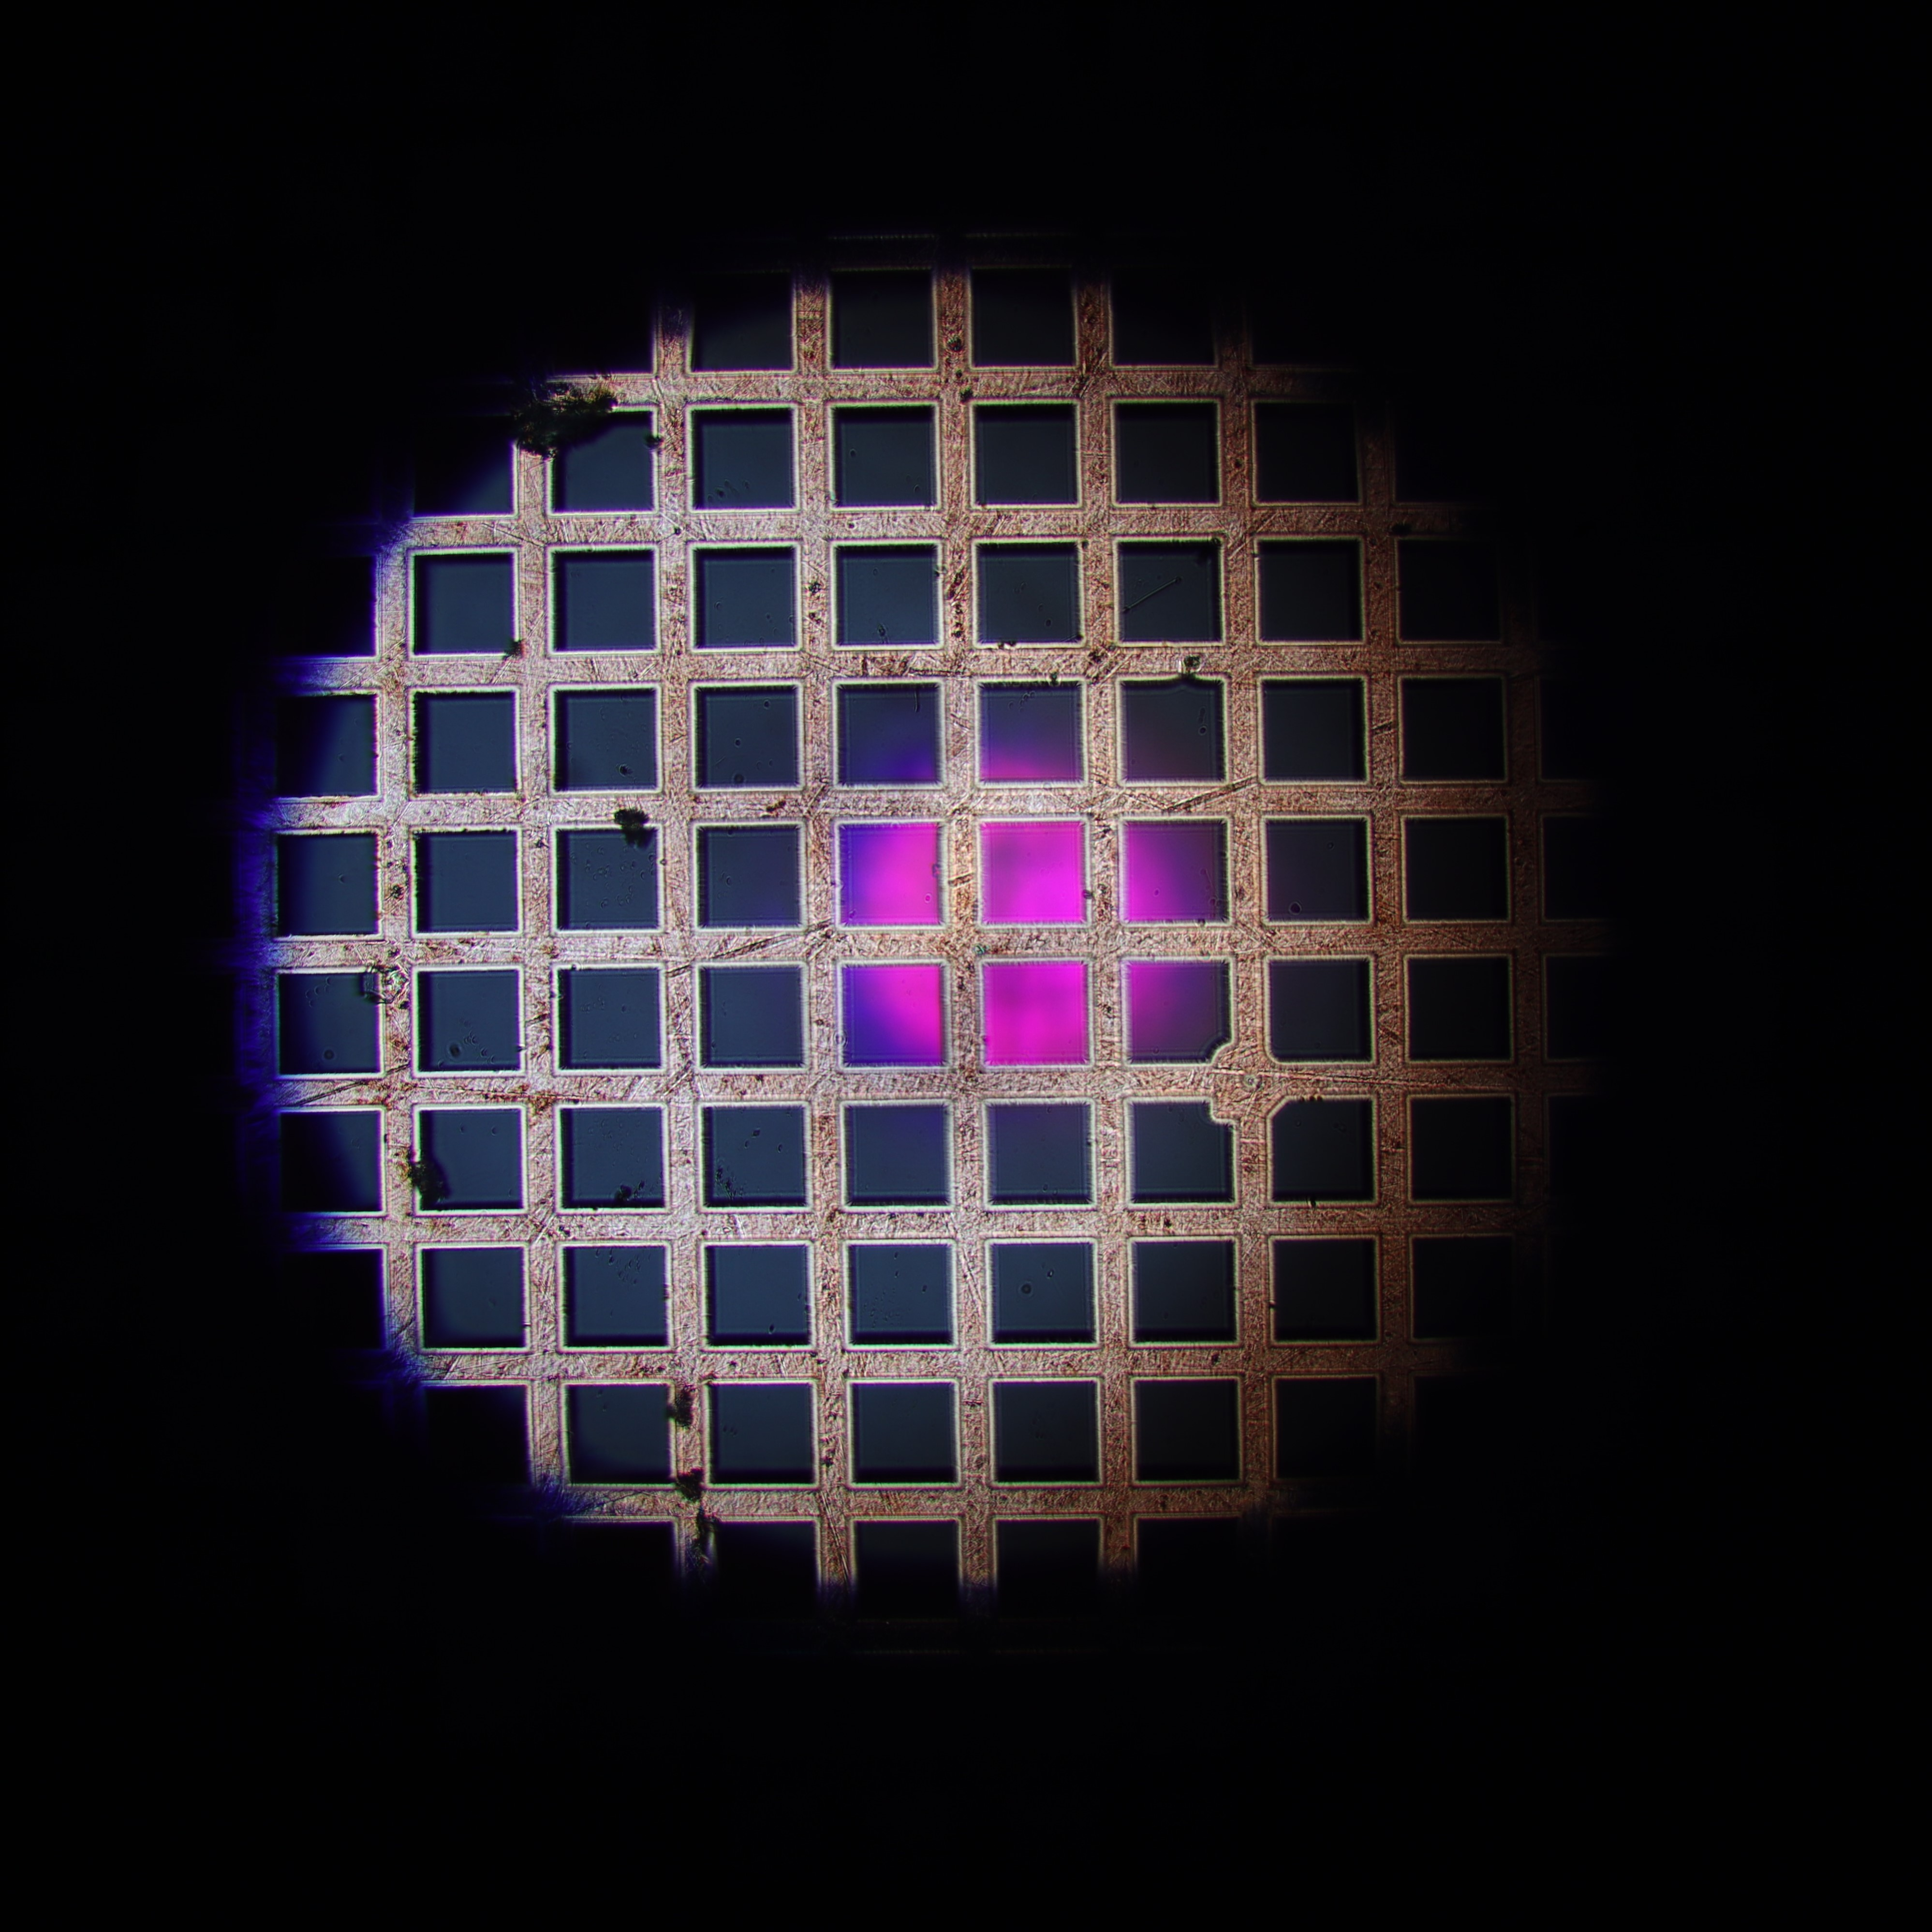
\includegraphics[width=0.5\linewidth]{om_off_brighest.JPG}
        \caption{OM: Coupled at brighest, collimated off BFP.}
        \label{figure: om_brightest_off}
    \end{figure}
    \subsubsection{較低亮度、匯聚於背焦面} \label{illuDark}
    為了避免上一個設定方式明顯的干擾紋路,我重新調整Coliimator,將光源匯聚至物鏡背焦面,並改為調整光纖的Coupler,以解決原初的設定中照明範圍不足的問題。在圖\ref{figure: evenest_on}、\ref{figure: om_evenest_on}中可以看見,
    經過調整後,照明關線的頻寬大幅減少,原先在\ref{section: illuOriginal}節中色相差的問題,幾乎完全消失,因此也確實可以完整的照明整個視野範圍,但由於實際進入光纖的光線已經減少許多,因此影像的整體亮度已有明顯的下滑。
    \begin{figure}
        \centering
        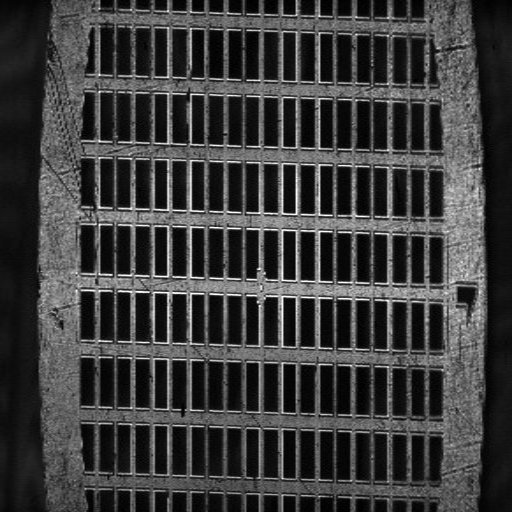
\includegraphics[width=0.5\linewidth]{on_evenest.jpg}
        \caption{Coupled at evenest, collimated off BFP.}
        \label{figure: evenest_on}
    \end{figure}
    \begin{figure}
        \centering
        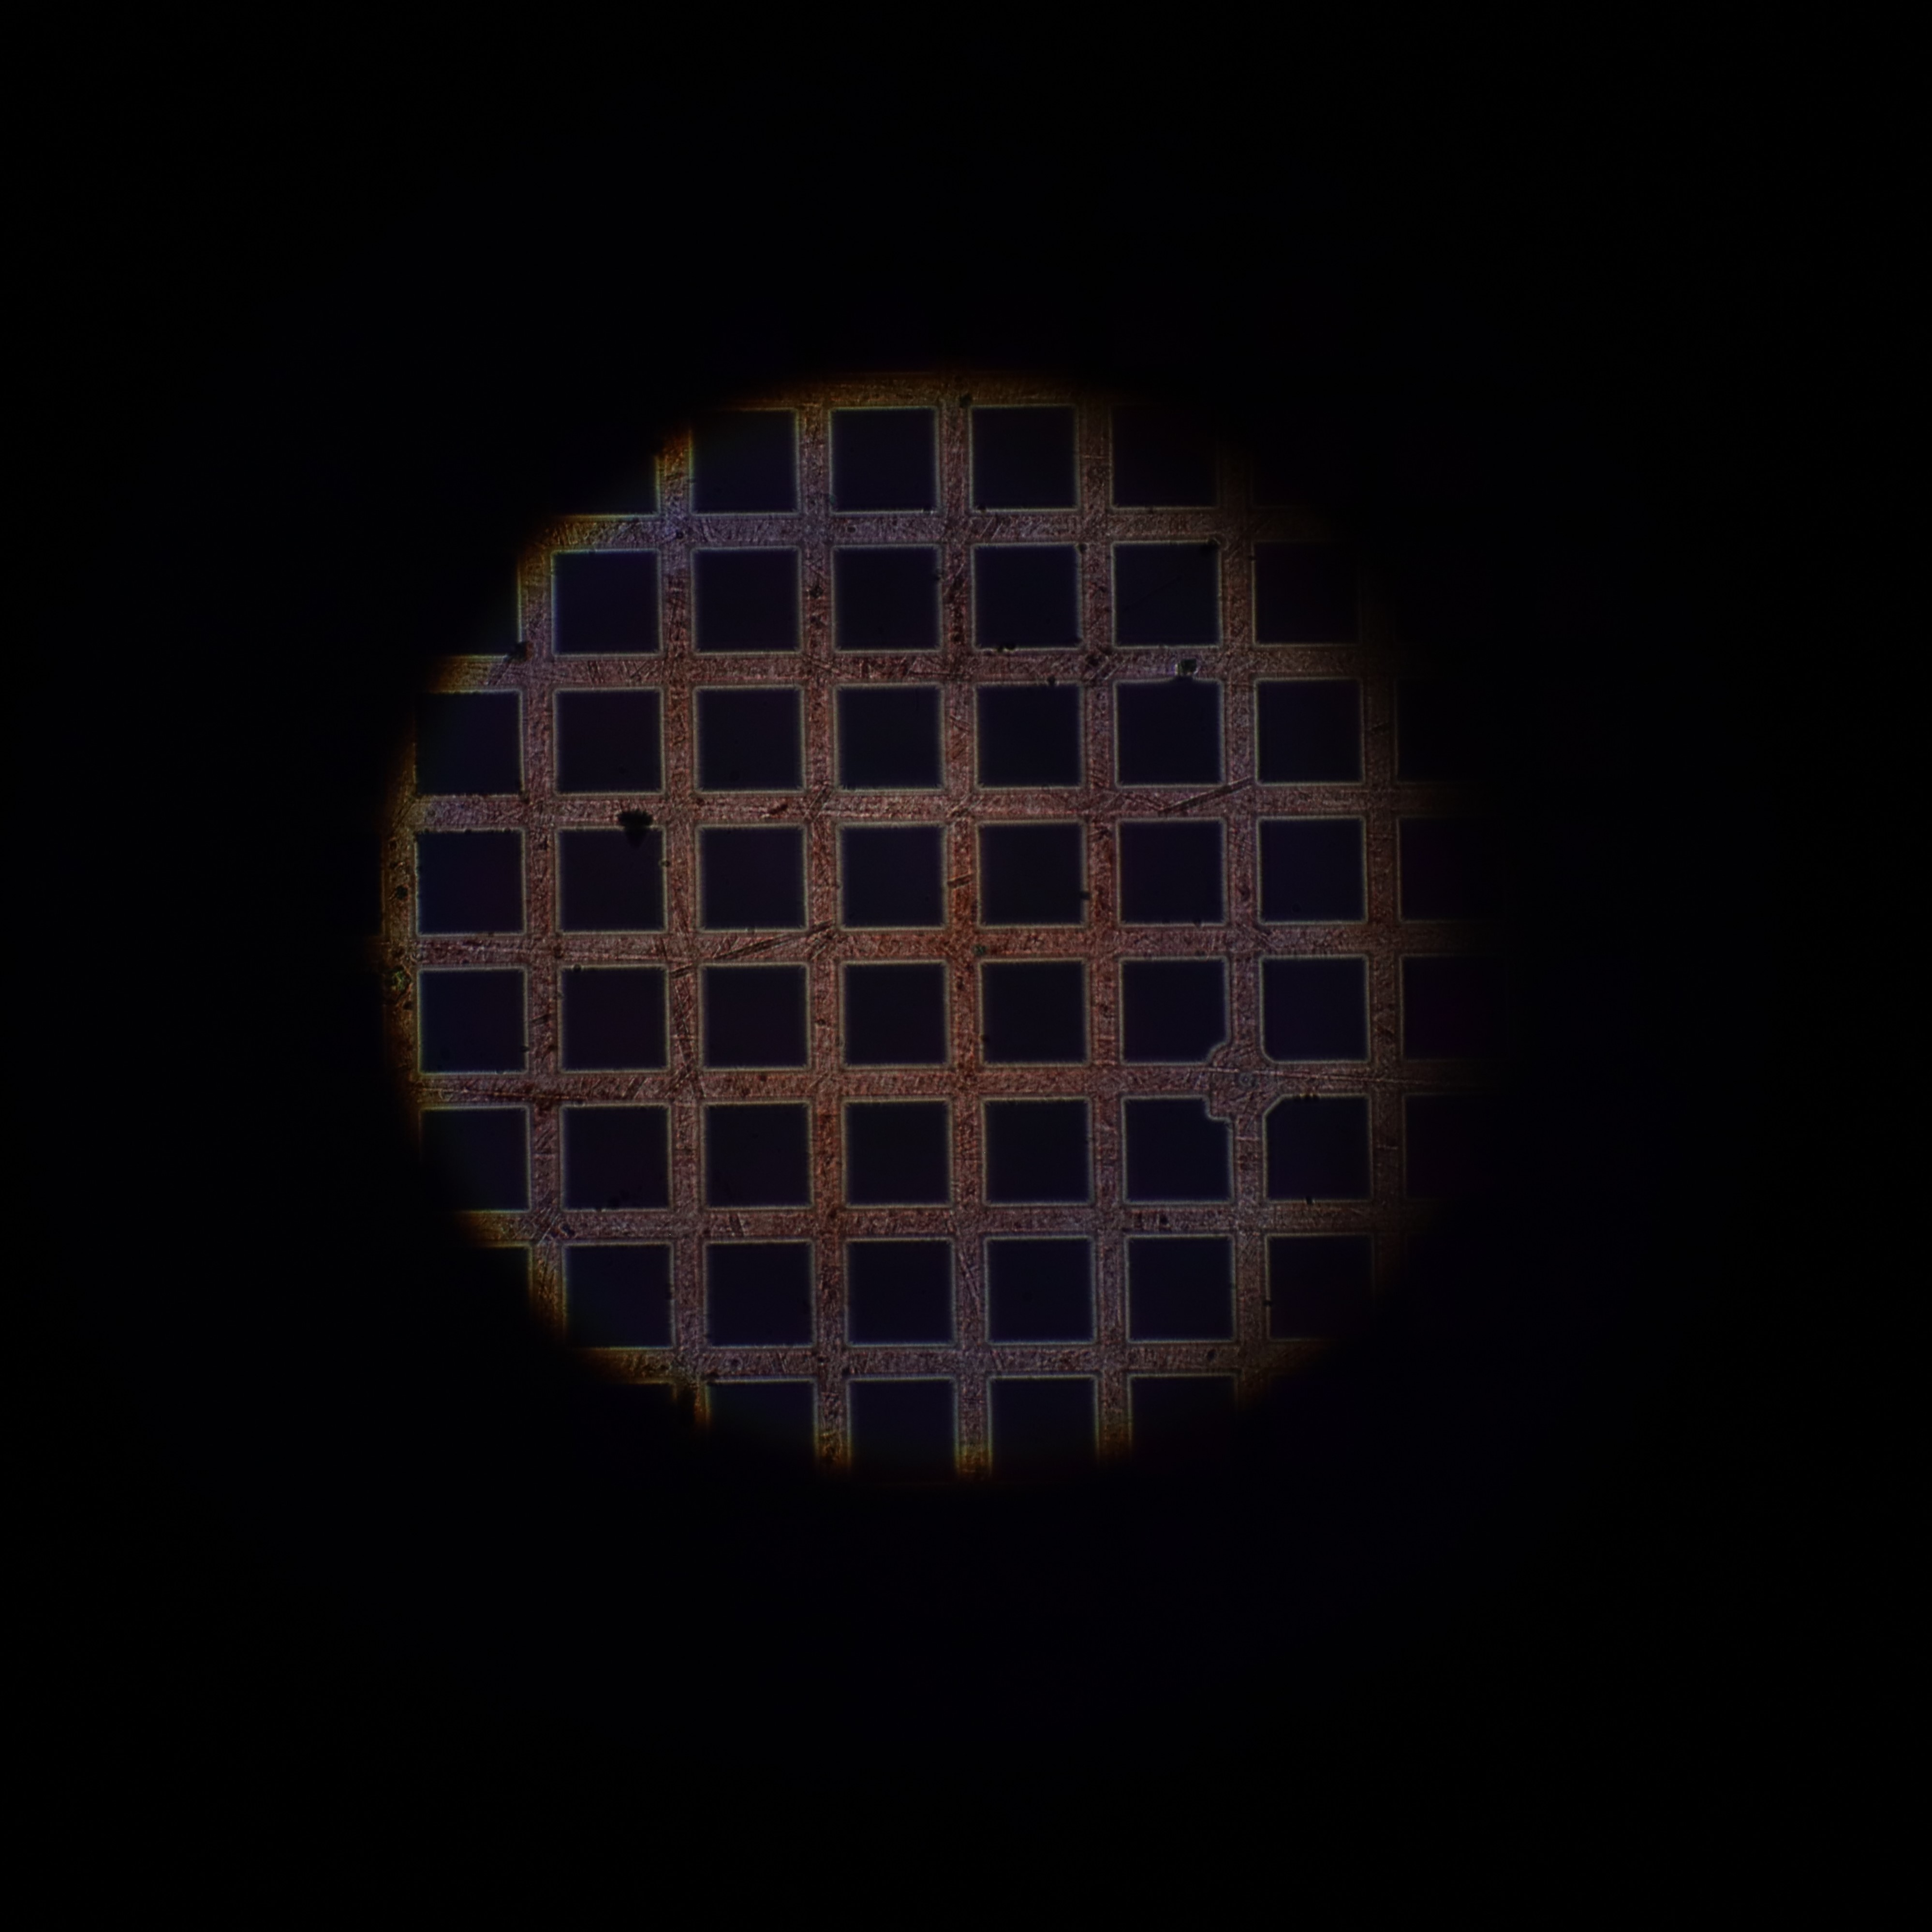
\includegraphics[width=0.5\linewidth]{om_on_evenest.JPG}
        \caption{OM: Coupled at evenest, collimated off BFP.}
        \label{figure: om_evenest_on}
    \end{figure}
    \newline \newline \noindent 綜上所述,照明的設定可以說是在光源光譜的完整度(頻寬)與照明範圍中做取捨,我們最後決定採取\ref{section: illuOriginal}節中的設定方式,
    雖然照明最後所得的影像會在上下有明顯的暗帶,但情形不算特別嚴重,且可以透過軟體進行後期處裡。若為了排除下上較暗的問題,而採取\ref{illuDark}的設定方式,形同於浪費了LDLS光源系統多數的光譜頻段,
    相形之下比上下的邊緣暗帶是更為嚴重問題,且也與我們因為需要更高頻寬的白光,而使用LDLS的初衷背道而馳。
    \section{第二階段: 軟體}
    \subsection{使用者介面}
    \subsection{.init檔}
    \subsection{軟體結構調整}
    
    \section{掃描速度}
\end{document}